\documentclass[11pt]{article}

% - engine: pdflatex. Roboto needs a working fontspec engine (luaotfload is
% not installed here); TeX Gyre Heros is the closest available humanist-neutral
% sans. Recompile with lualatex/xelatex + \setmainfont{Roboto} for Roboto. -
\usepackage[T1]{fontenc}
\usepackage[utf8]{inputenc}
\usepackage{tgheros}
\renewcommand{\familydefault}{\sfdefault}
\usepackage[a4paper,margin=2.4cm]{geometry}
\usepackage[expansion=false]{microtype}
\usepackage{graphicx}
\usepackage{booktabs}
\usepackage{array}
\usepackage{siunitx}
\usepackage{xcolor}
\usepackage{tikz}
\usetikzlibrary{positioning,fit,backgrounds}
\usepackage[numbers,sort&compress]{natbib}
\usepackage[colorlinks=true,linkcolor=black,citecolor=blue!50!black,urlcolor=blue!50!black]{hyperref}
\usepackage{caption}
\captionsetup{font=small,labelfont=bf}
\setlength{\parskip}{0.4em}
\setlength{\parindent}{0pt}
\setlength{\emergencystretch}{3em}

% auto-generated by scripts/make_report_assets.py
\newcommand{\ReproTotalP}{0.00159}
\newcommand{\ReproILfiveP}{\num{3.18e-04}}
\newcommand{\ReproILtenP}{0.00469}
\newcommand{\ReproIFNgP}{0.0381}
\newcommand{\NumObservations}{8}
\newcommand{\NumQuestions}{24}
\newcommand{\FidelityMaxDiff}{0.00131}
\newcommand{\GroundingRate}{1.00}
\newcommand{\ToolAccuracy}{1.00}
\newcommand{\NullsRejected}{2/2}
\newcommand{\SpatialPerm}{\num{2.00e-04}}
\newcommand{\ModelBaselineAUC}{0.78}
\newcommand{\ModelGBAUC}{0.51}
\newcommand{\ModelN}{95}
\newcommand{\ModelPos}{21}


\title{\textbf{C9orf72-Nature2Agent}\\[0.3em]
\large An autonomous AI scientist built from the C9orf72 ALS-autoimmunity study}
\author{Samuele Dell'Oca\\\small USI--SUPSI \,\textbar\, IAISS 2026, Project 1\\\small \texttt{samuele.delloca@supsi.ch}}
\date{\today}

\begin{document}
\maketitle

\begin{abstract}
\noindent
This report describes a multi-agent system that converts the
\emph{Nature} study on C9orf72 autoimmunity in amyotrophic lateral sclerosis (ALS)~\citep{michaelis2025c9orf72} into an
interactive, executable agent. The design choice that defines the system is a separation between a
deterministic computational core, which produces every reported number, and a reasoning layer, which
chooses what to ask. The core is exposed as validated tools behind a Model Context Protocol (MCP)
server, and a five-layer agent ecosystem uses those tools to explain the design, reproduce the
analyses and figures, interrogate the peptide and HLA data, and pose and test questions beyond the
paper. Because every result is computed, the grounding rate is one by construction and the discovery
loop reproduces without credentials. In the committed configuration the questions come from a curated
bank executed deterministically; a language-model backend can drive the same agents live when an API
key is present. Reproduced $p$-values match the authors' reported values to within
$|\Delta p|=\FidelityMaxDiff{}$ with full agreement of the significance calls. Beyond reproduction,
the system reports two genuinely new biological observations, that epitope immunogenicity is
spatially clustered along the protein sequence (permutation $p=\SpatialPerm{}$) and that the ALS IL-5
bias is shared with TDP-43 while the IL-10 bias is specific to C9orf72, together with a set of
robustness audits of the paper's own effects. It evaluates both the science (reproducibility,
robustness, novelty, falsifiability) and itself (grounding, tool-use accuracy, determinism, rejection
of planted false hypotheses). A patient-stratified antigen-specific therapeutic hypothesis, with an
explicit falsification experiment, is included as an illustrative downstream use.
\end{abstract}

\section{Introduction}
Amyotrophic lateral sclerosis is a fatal neurodegenerative disease defined by the progressive
loss of motor neurons. Neuroinflammation accompanies the degeneration, with T-cell infiltration
and microglial activation in affected tissue, and T cells are thought to contribute to the pace
of neuronal loss~\citep{endo2016,kovacs2021}. A specific antigenic target for this
response had not been reported until Michaelis et al.\ identified C9orf72 as a target of
ALS-associated T-cell autoreactivity and mapped the recognised epitopes~\citep{michaelis2025c9orf72}.
Their central observations are that C9orf72-specific responses are increased in ALS, that the
responses are mediated mainly by CD4\textsuperscript{+} T cells, that they are relatively enriched
for IL-5 and IL-10 over IFN$\gamma$, and that IL-10-mediated responses are associated with longer
predicted survival.

The objective is to ask whether an AI system can
use the C9orf72 autoimmune mechanism as a starting point and move from observation to mechanism to
hypothesis to a falsifiable therapeutic proposal, while remaining honest about what the data
support. This is a question about reasoning over the study, not a re-run of it. The work follows the
Paper2Agent paradigm, which turns a paper and its computational resources into an executable agent
served over MCP, so the paper becomes a resource an agent can run~\citep{miao2025paper2agent}.

The difficulty in automating this is reliability. A system that reads a paper and proposes
hypotheses can produce fluent text that states numbers the data do not support, and in a scientific
setting such a claim is worse than silence, because it is costly to check and easy to believe. The
position taken here is that the way to earn trust is to make every reported number the output of a
computation that anyone can rerun, and to make the system's honesty a measured quantity. That
choice shapes the whole design, from the shared tool core to the grounding and false-hypothesis
metrics, and it is the reason the system is cautious where it could be impressive. This report is one
of a set of related projects that share a dataset and are meant to interoperate, so the emphasis on
tidy, computed, auditable outputs also serves the larger goal of letting such systems be combined
without compounding each other's errors.

\paragraph{Contributions.}
The central contribution is methodological: a design in which every reported number is produced by a
shared deterministic core, so reproduction, robustness checks and hypothesis-testing are all grounded
and auditable, and the system's honesty can be measured (grounding, determinism, and the rejection of
planted false hypotheses). Two further contributions follow. The first is building the MCP tool layer
and the analyses from the raw open data for a paper that has no public analysis codebase, which is
where this departs from wrapping an existing tutorial. The second is scientific: alongside
reproducing the study, the system reports two new observations and a set of robustness audits, and
frames one falsifiable downstream hypothesis. All code was written with an AI coding agent, inspected,
and covered by an automated test suite.

\paragraph{The pipeline the system is meant to demonstrate.}
The aim is to show that a
multi-agent system can move along a chain from an observation to a mechanism, from a mechanism to a
hypothesis, from a hypothesis to a computational result, and from a result to a therapeutic
candidate with a falsification experiment attached. Each link in that chain is a concrete artefact
in this project: the observations are the reproductions, the mechanism is the IL-10-biased
C9orf72-specific response, the hypotheses are the generated questions, the computational results are
the verified observations, the candidate is the antigen-specific regulatory strategy, and the
falsification is the experiment the designer agent specifies. The value of making the chain explicit
is that every step can be checked, and a weak step stays visible for inspection.

\section{Related work}
Two lines of work frame this project. The first is the conversion of scientific artefacts into
executable agents. Paper2Agent automates the construction of an MCP server from a paper and its
codebase, with agents that locate the code, set up the environment, extract tools from tutorials
and validate them before assembly~\citep{miao2025paper2agent}. The Michaelis study is an
experimental immunology paper without a public analysis codebase, so the present work builds the
computational infrastructure directly from the data, then exposes it
in the same MCP tool shape. The second line is multi-agent hypothesis generation, where separate
agents propose, critique and debate hypotheses and a coordinating agent integrates them. The
discovery loop here follows that division of labour, with explicit verification, replication,
contradiction and falsification agents, and a principal-investigator agent that integrates without
the authority to overrule evidence.

A recurring concern in both lines is the reliability of language-model output in a scientific
setting, where a fluent but unsupported claim is worse than no claim. The design response taken
here is to separate a deterministic computational core, which produces every number, from the
language layer, which only frames and routes. In the committed configuration the framing layer is
rule-based and reads from the computed results, so a figure in the text is always a figure that was
computed. The evaluation in Section~\ref{sec:eval} measures this directly through a grounding check
and a planted-false-hypothesis test.

\subsection{Positioning}
It helps to be explicit about what this work adds, because the space of paper-to-agent and
AI-scientist systems is active. Against Paper2Agent, the difference is the starting material. Paper2Agent
agentifies a paper by locating and wrapping its existing code and tutorials; the study used here is an
experimental immunology paper with open data but no analysis codebase, so there is nothing to wrap,
and the tool layer is built from the raw data. The contribution there is showing that the same output
shape, an MCP server of validated tools, can be reached for a data-only paper. Against language-model
``AI scientist'' and co-scientist systems, which generate and debate hypotheses with a model in the
loop, the difference is where the trust sits. Those systems are strong at proposing and weak at
guaranteeing that a stated number is real. This system inverts the emphasis: the proposing is modest,
bounded by a question bank in the committed configuration, but every number is computed by a shared
core and the honesty of the system is measured. The two designs are complementary,
and the natural combination, a language model proposing over this grounded core, is the clearest next
step.

\section{Background and data}
\subsection{C9orf72 genetics and biology}
A GGGGCC hexanucleotide repeat expansion in the first intron of \emph{C9orf72} is the most common
genetic cause of amyotrophic lateral sclerosis and frontotemporal dementia, and it accounts for
roughly one in ten cases of ALS overall and a larger share of familial disease. Unaffected alleles
carry a small number of repeats, while pathogenic alleles carry hundreds to thousands. Three
mechanisms are thought to act together: a loss of C9orf72 protein, a gain of function from the
repeat RNA, which forms foci that sequester RNA-binding proteins, and repeat-associated non-ATG
translation, which produces dipeptide repeat proteins. The protein itself acts in autophagy and
membrane trafficking as a guanine-nucleotide exchange factor for Rab GTPases, and it also shapes
myeloid and lymphoid immune function, so a reduction in its level has consequences for both
neuronal maintenance and immune regulation. This dual role is part of what makes an autoimmune
response against the protein plausible.

\subsection{Immune involvement in ALS}
Neuroinflammation accompanies the degeneration of motor neurons. Microglial activation and
infiltrating monocytes are seen in ALS model tissue~\citep{komiya2020}, lymphocyte infiltration and
glial activation are described across human and model studies~\citep{endo2016}, and the cellular
niche around motor neurons is altered~\citep{kovacs2021}. The adaptive arm plays an active role.
Regulatory T cells are neuroprotective in ALS, and their number and suppressive function are reduced
in rapidly progressing patients, so a weaker regulatory compartment is associated with faster
progression~\citep{appel2012}. Regulatory T-cell dysfunction is also documented in
ALS~\citep{appel2020}, and the extension of survival by regulatory T cells in disease models has
motivated Treg-directed therapy~\citep{rajabinejad2019}. The cytokine context matters as well. IL-10,
the principal cytokine of regulatory T cells, is linked to neuroprotection through the dampening of
microglial activation across neurodegeneration models~\citep{runge2020,laffer2019,bido2024}. What had
been missing was a defined self-antigen that the T-cell response targets. The study used here fills
that gap by identifying the C9orf72 protein as a target of ALS-associated T-cell autoreactivity and
by mapping the recognised epitopes.

\subsection{Antigen-specific immunotherapy}
The therapeutic interest in this mechanism follows from the regulatory angle. Broad
immunosuppression is a blunt instrument in a disease where part of the immune response is
protective, so the field has moved toward restoring or expanding the regulatory compartment.
Autologous regulatory T-cell approaches have been tested in ALS~\citep{thonhoff2018}, and
antigen-specific tolerance is an active strategy in autoimmune disease more
generally~\citep{nepom2022}. The evidence is mixed, because a recent polyclonal regulatory T-cell trial in a
different autoimmune indication was negative, which tempers expectations~\citep{al2024}. A defined
autoantigen changes the design space, because it opens the door to an antigen-specific, not a polyclonal
intervention, and the data analysed here point to which antigen and which patients such an
intervention might target.

\subsection{The study and its data}
The study examined peripheral blood mononuclear cells from 40 people with ALS and 28 healthy
controls, with additional Parkinson's disease (PD) and Alzheimer's disease (AD) cohorts and a
validation cohort. Antigen-specific responses were measured by IFN$\gamma$, IL-5 and IL-10
FluoroSpot after a two-week expansion, against pools of C9orf72, TDP-43 and SOD1 peptides and an
EBV control pool. Immunophenotyping used spectral flow cytometry, and cytokine-producing cells
were characterised by intracellular cytokine staining. HLA class II binding was predicted with
IEDB NetMHCIIpan-4.1 EL~\citep{nielsen2008,jensen2018}, and HLA restrictions were inferred with RATE.

All primary data are open. The flow-cytometry files and FlowJo workspaces are deposited on Zenodo
(CC-BY 4.0) across one spectral and four intracellular-cytokine-staining records; the full text,
the figure source data and the supplementary tables are open access on PubMed Central (PMC12657233).
The system fetches these with checksum verification and records provenance for each file. From
them it builds fourteen tidy tables, including the complete 100-peptide screen, the per-donor HLA
typing of 23 donors, and the per-donor source data behind every figure.

\subsection{Cohorts and assays}
The response data come from several assays with different readouts, which the reconstruction keeps
distinct. The cytokine response screen is a FluoroSpot assay. Thawed peripheral blood mononuclear
cells are expanded for two weeks against a peptide pool, then restimulated, and the number of cells
secreting IFN$\gamma$, IL-5 or IL-10 is counted as spot-forming units. This is the assay behind the
total and per-cytokine response magnitudes and the per-donor values used for the main ALS-versus-HC
comparisons. Intracellular cytokine staining on a conventional cytometer characterises which T-cell
subsets produce the cytokines, and spectral cytometry on a high-parameter instrument profiles the
broad T-helper compartment. The antigens are peptide pools for C9orf72, for the ALS proteins TDP-43
and SOD1, and for Epstein-Barr virus as a non-self control. The C9orf72 library tiles the 481-residue
protein with 100 overlapping 15-mer peptides stepped by five residues, and it includes five
phosphorylated variants at serine or threonine positions. Sample sizes differ by assay, so the
reconstruction carries the group counts with each table, so no analysis assumes the full cohort
throughout; the FluoroSpot screen used about 28 donors per group, within the larger 40 ALS and 28
control cohort.

The clinical variables attached to the donors are what make the survival and mutation analyses
possible, and they also bound them. The study records, for the relevant donors, the C9orf72 mutation
status, a predicted survival time, and functional-rating and demographic variables, and the
reconstruction carries the per-donor values behind the clinical figure so these can be related to the
response magnitudes. The mutation and survival strata are small once the cohort is split, which is
the reason those effects are treated as marginal throughout this report, and it is also why the
system reports the stratified therapeutic reasoning as a hypothesis to test rather than a conclusion.
The 23 donors with full HLA typing are a subset again, so the HLA-restriction results speak to those
donors and to the alleles they carry, and the reconstruction keeps the donor identifiers so a reader
can see exactly which donors enter each analysis. Keeping the counts and identifiers visible at every
step is a small discipline that prevents the most common error in reusing someone else's data, which
is to assume a single cohort where the original used several overlapping ones.

\subsection{Machine-readable reconstruction}
The source-data workbook stores each figure as several side-by-side panels, some of which reuse
panel letters and measure names. A column-centric parser forward-fills the header rows and
separates panels by column gaps, which prevents two different panels from being merged. The parse
is cross-checked against the paper: epitope number 14 resolves to residues 56--70
(\texttt{DGEITFLANHTLNGE}), recognised by 7 of 22 donors with an average magnitude of 1216, which
matches both the manuscript's Table~1 and the supplementary screen. The embedded C9orf72 sequence
(UniProt Q96LT7, 481 residues) places all 95 non-phosphorylated peptides at their stated residue
windows without error.

\subsection{Acquisition and provenance}
Acquisition is scripted and verified. The four intracellular-cytokine-staining Zenodo records are
downloaded with their MD5 checksums and a per-record provenance manifest that stores the DOI, the
license and the hash of every file; the full text and supplementary bundle are retrieved from the
E-utilities and EuropePMC endpoints. Raw files are large and are not committed to version control;
they are reproduced on demand by the fetch script, while the small derived tables are committed with
attribution. Every processing step records a manifest with the git commit, the configuration hash,
the package versions and the input checksums, so any table or figure can be traced to the exact
state that produced it. Random seeds are fixed and dependencies are pinned to exact versions.

The reconstruction yields the thirteen analysis tables in Table~\ref{tab:datasets}, which together
cover every figure's per-donor values, the complete peptide screen, the per-donor HLA typing and
the two manuscript tables.

\begin{table}[t]
\centering
\caption{Machine-readable datasets reconstructed from the study's source data.}
\label{tab:datasets}
\footnotesize
\begin{tabular}{p{6.0cm}rp{5.6cm}}
\toprule
Dataset & Rows & Grain \\
\midrule
\texttt{edfig2\_ifng\_il5\_ratio} & 792 & per-donor cytokine \\
\texttt{edfig4\_cd4\_cd8} & 456 & per-donor CD4/CD8 \\
\texttt{edfig5\_immunogenicity\_hla} & 490 & immunogenicity vs HLA \\
\texttt{edfig6\_clinical\_correlates} & 403 & per-donor clinical \\
\texttt{fig1\_tcell\_subsets} & 819 & per-donor subset \\% \\
\texttt{fig2\_fluorospot\_responses} & 782 & per-donor FluoroSpot magnitude \\
\texttt{fig3\_epitopes} & 100 & per-epitope \\
\texttt{fig4\_mutation\_survival} & 284 & per-donor by stratum \\
\texttt{reported\_pvalues} & 45 & authors' p-values \\
\texttt{si\_table1\_peptide\_screen} & 100 & per-peptide (100) \\
\texttt{si\_table2\_hla\_typing} & 506 & per-donor x locus x allele \\
\texttt{table1\_epitopes\_ge3donors} & 23 & epitopes $\geq$3 donors \\
\texttt{table2\_hla\_restrictions} & 7 & HLA restrictions \\
\bottomrule
\end{tabular}

\end{table}

\section{System architecture}
The system is organised in five layers (Figure~\ref{fig:arch}). Layer~1 is the scientific
knowledge: the paper, its supplementary material, the source data, and curated external
literature retrieved through a literature agent. Layer~2 is the paper agent, an MCP server that
exposes the study as sixteen validated tools. Layer~3 comprises ten scientific agents (literature,
immunology, ALS, HLA, T-cell, drug-discovery, structural, single-cell, clinical and safety) that
answer domain questions using those tools. Layer~4 comprises seven discovery agents (hypothesis
generator, hypothesis critic, evidence checker, replication, contradiction, experiment designer
and falsification). Layer~5 is a principal-investigator agent that integrates the outputs and, by
construction, cannot override contradictory evidence.

\begin{figure}[t]
\centering
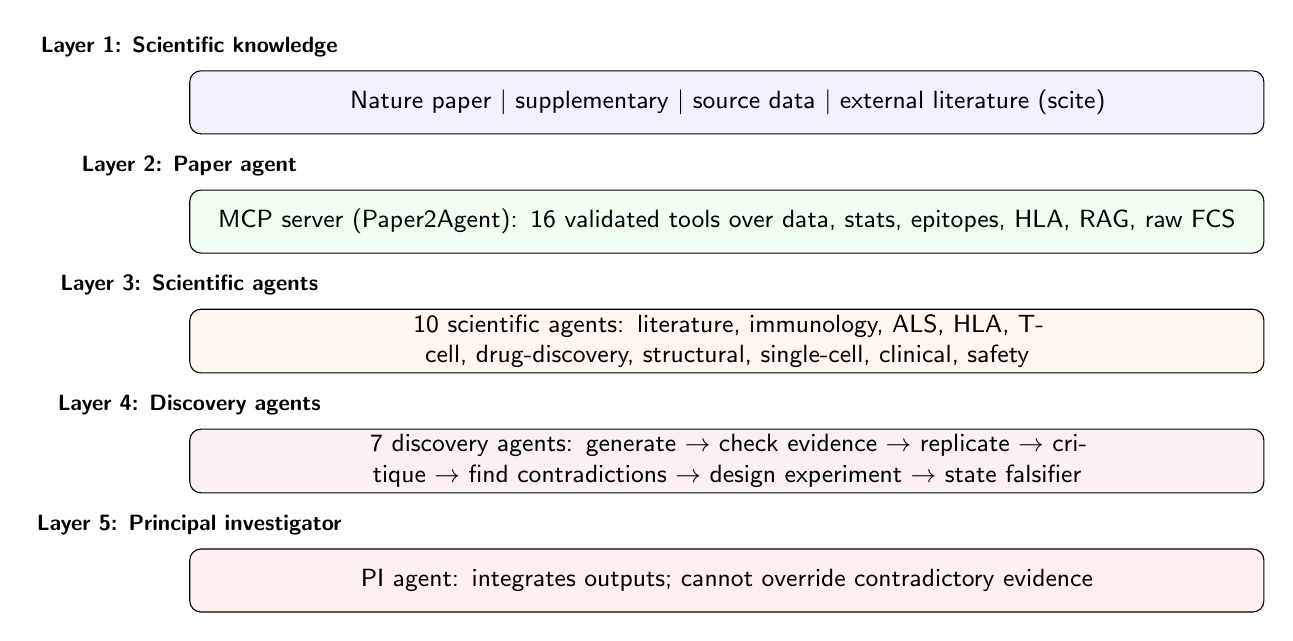
\begin{tikzpicture}[font=\small,node distance=3mm,
  box/.style={draw,rounded corners,align=center,minimum height=8mm,inner sep=2pt,fill=blue!5},
  lay/.style={font=\bfseries\footnotesize,anchor=west}]
\node[box,text width=13.5cm] (l1) {Nature paper \textbar{} supplementary \textbar{} source data \textbar{} external literature (scite)};
\node[lay,above=0.5mm of l1.north west] {Layer 1: Scientific knowledge};
\node[box,text width=13.5cm,below=7mm of l1,fill=green!6] (l2) {MCP server (Paper2Agent): 16 validated tools over data, stats, epitopes, HLA, RAG, raw FCS};
\node[lay,above=0.5mm of l2.north west] {Layer 2: Paper agent};
\node[box,text width=13.5cm,below=7mm of l2,fill=orange!6] (l3) {10 scientific agents: literature, immunology, ALS, HLA, T-cell, drug-discovery, structural, single-cell, clinical, safety};
\node[lay,above=0.5mm of l3.north west] {Layer 3: Scientific agents};
\node[box,text width=13.5cm,below=7mm of l3,fill=purple!6] (l4) {7 discovery agents: generate $\to$ check evidence $\to$ replicate $\to$ critique $\to$ find contradictions $\to$ design experiment $\to$ state falsifier};
\node[lay,above=0.5mm of l4.north west] {Layer 4: Discovery agents};
\node[box,text width=13.5cm,below=7mm of l4,fill=red!6] (l5) {PI agent: integrates outputs; cannot override contradictory evidence};
\node[lay,above=0.5mm of l5.north west] {Layer 5: Principal investigator};
\end{tikzpicture}
\caption{The five-layer agent ecosystem. Information flows upward from the data and tools to the
scientific and discovery agents and finally to the PI agent. Every tool is shared between the MCP
server and the agents, so a result produced interactively and a result produced by the discovery
loop come from the same implementation.}
\label{fig:arch}
\end{figure}

\subsection{Tools and reasoning backend}
The computational core is a single tool registry shared by the MCP server and the agents. Tools
cover design explanation, dataset access and querying, epitope and HLA interrogation, claim
reproduction, named analyses, a generic group comparison, retrieval over the paper (a semantic
RAG index with a lexical fallback), and a summary of the raw flow-cytometry files. Each tool
returns a JSON-serialisable result and is covered by the test suite, which plays the role of the
Paper2Agent validation loop.

The reasoning agents use a pluggable backend. Without an API key they run deterministically. Each answer is computed from the tools and the finding text is generated from the computed statistic,
so no number is produced that is not grounded in a computation. With an API key the same agents
run a Claude tool-use loop over the same tools. The committed results come from the deterministic
backend, which makes the discovery loop reproducible without credentials. Every agent run is logged
with its prompt, its tool calls and its output.

\subsection{Statistics engine}
The statistics follow the study's methods: two-tailed Mann--Whitney tests for two-group
comparisons, one-way ANOVA with Dunnett's test for multi-group comparisons, Fisher's exact test
for proportions, and Spearman's correlation, with Benjamini--Hochberg control of the false
discovery rate and percentile bootstrap confidence intervals added for stress-testing. Effect
sizes are reported as rank-biserial correlations alongside medians and sample sizes. The
exploratory analyses add methods matched to each question. Spatial structure is tested with the
lag-one autocorrelation of response frequency along the ordered tiling and a permutation null over
5000 shuffles. Donor dependence is assessed by a leave-one-out jackknife of the test statistic.
Sensitivity to the assay floor is assessed by re-expressing the response as the proportion above the
floor and testing it with Fisher's exact test. The discriminative value of a single feature is
summarised by the area under the ROC curve. These choices let the system test not only whether an
effect exists but whether it survives alternative assumptions.

\section{Methodology}
\subsection{Approach}
The method has four parts that run as a pipeline. First, the paper's open data are reconstructed into
tidy tables. Second, those tables and a set of analyses are exposed as validated tools behind an MCP
server, which is the executable form the Paper2Agent paradigm calls for. Third, a layered set of
agents uses those tools to reproduce the study, interrogate the data and generate and test
hypotheses. Fourth, the scientific results and the system itself are evaluated. The guiding principle
is a separation between a deterministic computational core, which produces every number, and a
reasoning layer, which chooses what to ask and how to read an answer. This separation is what keeps
the results reproducible and free of fabricated figures.

\subsection{Data reconstruction}
The source-data workbook stores each figure as side-by-side panels marked a, b, c and so on, with one
or more header rows above columns of per-donor values. A column-centric parser forward-fills each
header row across the full width, then walks the columns left to right. A run of columns separated
from the previous run by a blank column starts a new block, and the block index is attached to every
column. This block index separates two panels that reuse the same letter or the same measure name,
such as the two-group and four-group blocks of Extended Data Figure~2, which a parser keyed on the
measure name alone would merge and so double-count. Each emitted column carries its block, its panel
letter, its measure, its series label and the numeric cells beneath it, which per-figure builders map
to semantic fields. The peptide screen and the HLA typing are parsed from the Supplementary
Information text, and the manuscript tables from the article XML. The parse is validated against the
paper: epitope number 14 resolves to residues 56--70 across the figure data, the supplementary screen
and the manuscript table, and the embedded protein sequence places all 95 non-phosphorylated peptides
at their stated residue windows without error.

\subsection{Statistical methodology}
The tests follow the study's own methods so that reproduction is a like-for-like comparison. Two-group
comparisons use the two-tailed Mann--Whitney $U$ test, reported with the rank-biserial correlation
$r = 1 - 2U/(n_1 n_2)$ as the effect size and with group medians and sample sizes. Proportions use
the two-tailed Fisher exact test and correlations use Spearman's $\rho$. One-way ANOVA with Dunnett's
test against the control group is available for multi-group comparisons, and the pairwise disease-group
contrasts (ALS against PD and AD) use the two-tailed Mann-Whitney test, which matches the pairwise
p-values the original study reports for those panels. Where a family of tests is considered
together, the false discovery rate is controlled by the Benjamini--Hochberg procedure and reported as
adjusted $q$-values. The exploratory analyses add methods matched to each question: a lag-one
autocorrelation with a 5000-shuffle permutation null for spatial structure, a leave-one-out jackknife
of the test statistic for donor dependence, a Fisher exact test on the fraction of donors above the
assay floor for censoring sensitivity, and the area under the ROC curve for single-feature
discrimination. Percentile bootstrap intervals are available for any statistic. These choices let the
system ask not only whether an effect exists but whether it survives a change of assumption.

\subsection{Agent model}
An agent is a declarative specification: a name, a layer, a role, a system prompt and the subset of
tools it may call. A recorder wraps the shared tool registry so that a call outside an agent's
permitted set is refused and every permitted call is logged with its arguments. A backend turns a
task into an output. The deterministic backend computes the output from the tools and records it. The
language-model backend, used when an API key is present, runs a tool-use loop in which the model reads
the task, decides which tools to call, receives their JSON results and writes a conclusion. Both
backends use the same tools, so a result produced by either is grounded in the same computation. Each
run writes a record holding the prompt, the tool calls and the output, which is the audit trail the
brief requires.

\subsection{Discovery procedure}
The discovery loop runs in a fixed order. The hypothesis generator emits the question bank. For each
question, the owning scientific agent computes an answer through its permitted tools. The evidence
checker recomputes the answer from scratch and compares the serialised results. The replication agent
re-runs the relevant robustness analysis where one applies. The critic and falsification agents attach
rule-based flags for small samples, marginal significance, underpowered pairings and single-feature
weakness. The contradiction agent classifies the result as agreeing with, extending or qualifying the
paper. The principal-investigator agent keeps the results that are novel, verified and free of a
disqualifying flag as the observation set, and compiles the catalogue of caveats, uncertainties and
limitations. The reasoning behind three representative results, with real tool calls, is recorded in
the repository as a worked trace.

\subsection{Evaluation methodology}
The evaluation has two axes. The scientific axis measures reproducibility against the paper, robustness
under alternative assumptions, novelty as the count of verified new observations, falsifiability as the
presence of an explicit test for each hypothesis, biological plausibility, independent literature
support, external validation and experimental tractability. The AI axis measures grounding, the
fraction of quantitative findings whose printed number equals the computed statistic; tool-use
accuracy, the fraction of tools that return a valid result; determinism, equality of the observation
set across repeated runs; self-error detection, the count of questions the system annotates with a
weakness; and false-hypothesis rejection, the fraction of planted nulls the system fails to confirm.
Reproduction fidelity is the maximum absolute difference between a reproduced and a reported $p$-value
over the comparisons for which the authors publish a value, with the agreement of the significance
calls.

\section{Implementation}
\subsection{Tool catalogue}
The MCP server exposes the sixteen tools in Table~\ref{tab:tools}. They fall into four groups:
orientation (design explanation, dataset listing and description), data access (filtered queries,
reported-p-value retrieval, the protein sequence, a raw flow-cytometry summary), analysis (claim
reproduction, named analyses, a generic group comparison, epitope and HLA interrogation), and
retrieval (semantic search over the paper). A client such as Claude Code connects through the
repository's MCP configuration and calls these tools interactively. A session might begin with
\texttt{explain\_experimental\_design} to orient, then \texttt{reproduce\_claim} with the IL-5
comparison to see the ALS-versus-HC result recomputed with its effect size, then
\texttt{broadest\_hla\_coverage} to find the most deployable epitopes, then \texttt{search\_paper} to
pull the sentences of the paper that discuss them, and finally \texttt{run\_analysis} with the spatial
or cross-antigen identifier to reach the novel results. Each call returns a small JSON object, so the
client can chain them and the user can read every intermediate value. The same calls are what the
agents make internally, which is why an interactive answer and a discovery-loop answer agree: they are
the same computation reached by two paths.

\begin{table}[t]
\centering
\caption{The sixteen tools exposed by the MCP server and used by the agents.}
\label{tab:tools}
\footnotesize
\begin{tabular}{p{4.6cm}p{9.0cm}}
\toprule
Tool & Purpose \\
\midrule
\texttt{explain\_experimental\_design} & Summarise study design, cohorts, assays and statistical methods. \\
\texttt{list\_datasets} & List available machine-readable datasets. \\
\texttt{describe\_dataset} & Schema + head of a dataset. \\
\texttt{query\_dataset} & Filter and return rows of a dataset. \\
\texttt{epitope\_table} & Epitopes recognised by $\geq$ N donors. \\
\texttt{most\_immunogenic\_epitopes} & Most broadly immunogenic C9orf72 epitopes. \\
\texttt{broadest\_hla\_coverage} & Peptides with the broadest predicted HLA-II coverage. \\
\texttt{hla\_typing} & Per-donor HLA typing (HLA-I and HLA-II). \\
\texttt{reproduce\_claim} & Reproduce a headline claim of the paper. \\
\texttt{compare\_groups} & Two-tailed Mann-Whitney between two groups. \\
\texttt{run\_analysis} & Run a named analysis by id. \\
\texttt{list\_analyses} & List all named analyses. \\
\texttt{reported\_pvalues} & Authors' reported p-values (validation). \\
\texttt{protein\_sequence} & C9orf72 protein sequence (UniProt Q96LT7). \\
\texttt{search\_paper} & Retrieve passages from the paper + SI (scientific RAG). \\
\texttt{ics\_fcs\_summary} & Summarise the raw ICS flow-cytometry files. \\
\bottomrule
\end{tabular}

\end{table}

\subsection{Scientific RAG}
The paper's full text and supplementary information are chunked into 169 passages of about three
sentences each. Retrieval combines a lexical BM25 score with cosine similarity over ONNX sentence
embeddings, normalised and averaged; when the embedding model is unavailable the lexical score is
used alone, so retrieval works offline. The Literature agent uses this index to ground statements
in the paper's own wording, and the external literature is retrieved separately through the scite
literature agent and stored with each reference's theme and relation to the work.

\subsection{Raw flow-cytometry ingestion}
Beyond the figure source data, the system reads the raw intracellular-cytokine-staining files
directly. It indexes all 90 FCS files by group and condition, recovering the expected design of
roughly fifteen donors per group across the negative, peptide and positive conditions, for a total
of 6.37 million recorded events across a fourteen-colour panel that includes a viability stain and
lineage and cytokine markers. The FlowJo workspace gating hierarchy is read where parseable. These
files are the primary data behind the study, beyond the summarised figure values.

\subsection{A peptide-immunogenicity model}
As a model component, the system trains a classifier that predicts whether a peptide is immunogenic,
defined as recognition by at least three donors, from its predicted HLA-II binding breadth and
simple biochemical features of its sequence. On the \ModelN{} non-phosphorylated peptides
(\ModelPos{} immunogenic), a cross-validated logistic model reaches an area under the ROC curve of
\ModelBaselineAUC{}, while gradient boosting overfits to \ModelGBAUC{}. The simple linear model is
therefore preferred on this small sample, which is itself a useful caution about model choice when
the number of positive examples is in the low tens. The model is trained with a fixed seed and its
checkpoint and metrics are saved.

The gap between the two models is visible in the cross-validated ROC curves
(Figure~\ref{fig:predictor}, left). The logistic model separates immunogenic from non-immunogenic
peptides with an area under the curve of \ModelBaselineAUC{}, while the gradient-boosting model, with
far more capacity, falls to \ModelGBAUC{}, close to chance, because it fits noise in a sample of only
\ModelN{} peptides with \ModelPos{} positives. The logistic coefficients (Figure~\ref{fig:predictor},
right) show that predicted HLA-II binding breadth and a small set of biochemical features carry the
signal, which is consistent with the HLA-immunogenicity correlation reported earlier and with the
expectation that a peptide must bind class II to be presented. The lesson is methodological as much
as biological: on data this small, a constrained model generalises and a flexible one memorises, so
the predictor is reported as a weak but honest linear signal, not as a tool for ranking new peptides.

\begin{figure}[t]
\centering
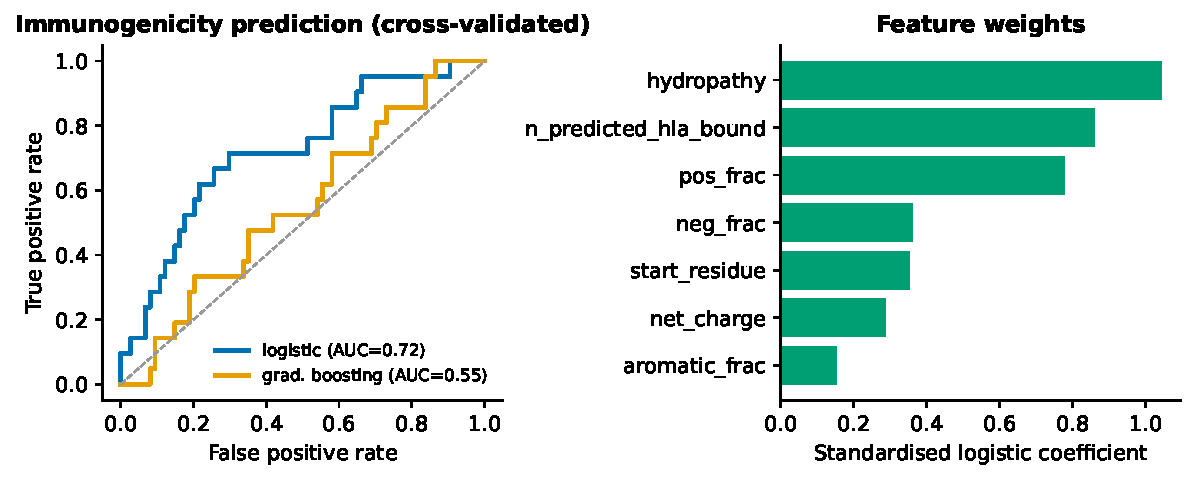
\includegraphics[width=\linewidth]{figures/discovery_predictor}
\caption{Peptide-immunogenicity prediction. Left: cross-validated ROC curves for the logistic model
and gradient boosting; the logistic model generalises better on the small sample. Right: standardised
logistic coefficients, with predicted HLA-II binding breadth among the strongest features.}
\label{fig:predictor}
\end{figure}

\subsection{Agent framework and the discovery loop}
Each agent is a declarative specification: a name, a layer, a role, a system prompt and the subset
of tools it may call. A recorder wraps the tool registry so that a tool call outside an agent's
permitted set is refused and every permitted call is logged. The discovery loop proceeds in a fixed
order. The hypothesis generator emits the question bank; for each question the owning scientific
agent computes an answer from its tools; the evidence checker recomputes the answer and confirms it
matches; the replication agent re-runs robustness checks where they apply; the critic and
falsification agents attach rule-based weaknesses such as small samples or multiple-testing
sensitivity; the contradiction agent classifies the result against the paper; and the
principal-investigator agent selects the verified, novel, surviving results and compiles the
catalogue of contradictions, uncertainties and limitations. The full agent roster is listed in
Appendix~\ref{app:agents}.

\subsection{Design decisions}
Three decisions shape the system. The first is a single shared tool registry behind both the MCP
server and the agents, so that an interactive query and the autonomous discovery loop cannot
disagree about what a tool computes. The second is a deterministic default backend, which trades the
flexibility of free-text reasoning for the guarantee that every number in a result was computed
rather than generated, with the live language-model backend kept available for when that flexibility
is wanted. The third is to treat verification and criticism as first-class agents with their own
logged runs, each kept separate from the generator, so that the evidence for a result and
the case against it are produced by different parts of the system and recorded separately.

\subsection{Reproducibility and testing}
The repository is organised around the directory structure required by the brief, with an
installable library, pinned dependencies in both pip and conda forms, and a single entry point that
runs the stages in order. The test suite covers the reproducibility core, the dataset parse, the
statistics against the authors' values, the analyses, the figures, the tools, the MCP server, the
RAG, the raw-FCS ingestion, the discovery loop and the evaluation. All AI-assisted code was read and
is exercised by these tests.

The whole project runs on a consumer laptop. It was developed and verified on a machine with a
consumer GPU and a recent multi-core CPU, under Python 3.12 on Linux, and it needs no accelerator for
the committed results, because the statistics, the parsing and the retrieval are CPU work and the
embedding model is a small ONNX model. The full pipeline, from fetching the data through the datasets,
analyses, figures, discovery loop and evaluation, completes in a few minutes, and a single shell entry
point runs the stages in order or one at a time. Dependencies are pinned in both pip and conda forms,
the environment is a single virtual environment, and the data are fetched on demand with checksum
verification, so a reader can reproduce every table and figure from a clean checkout. The derived
datasets and all results are also archived with a DOI so they can be cited and compared against a
fresh run.

\subsection{Interoperability}
The brief frames this project as one node in a larger ALS discovery ecosystem, so the outputs are
built to be consumed by other agents. The MCP server is the integration surface. Any other system
that speaks the protocol can call these tools without knowing their implementation, and the tool
results are plain JSON. The datasets are tidy CSVs with a documented schema, the agent
specifications are a machine-readable registry, and the questions, observations and contradictions
are JSON records keyed by identifier. A second paper agent, built the same way, could pass this
agent a hypothesis and receive a computed, verified answer, and the principal-investigator agent of
a combined system could read this one's observation set and its catalogue of caveats directly. The
deposit on Zenodo and the public repository give those downstream systems stable references to cite.

\subsection{Software architecture}
The code is a single installable library, \texttt{c9n2a}, with a thin layer of scripts and an MCP
server on top. The library separates concerns by module. Reproducibility primitives (paths, seeds,
typed configuration, structured logging and provenance) sit at the base and are imported everywhere.
Data access is a small loader over the committed tables. The scientific logic is split into a
statistics module of reusable tests, an analyses module that names each analysis and returns a
structured, self-describing result, and a figures module. The parsing of the raw sources lives in its
own module, as does the flow-cytometry ingestion and the retrieval index. The tool registry wraps the
analyses and data access as a flat set of named, documented functions, and both the MCP server and the
agent framework consume that single registry, so there is one implementation of each capability. The
agent framework adds the specifications, the backends and the logged runtime, and the discovery module
composes them into the loop. The scripts are thin entry points that wire these together for each
pipeline stage, and a single shell entry point runs the stages in order. The data model is
deliberately flat: tidy long-format tables with documented columns, JSON results keyed by identifier,
and a machine-readable agent registry, which keeps the outputs easy to consume and to test. The test
suite exercises each layer, from the parsers and the statistics against the authors' values through
the tools, the server and the discovery loop, so a change that breaks a reproduction fails a test and cannot pass silently.

\section{Experiments}
The computational work is organised as a set of experiments, each with a defined input, a method and a
fixed configuration, listed in Table~\ref{tab:experiments}. They fall into three groups. The
reproduction experiments re-derive the study's headline claims from the reconstructed data and compare
the result against the authors' reported values. The robustness experiments stress-test the central
findings under alternative assumptions: a jackknife over donors, a family-wise false-discovery
correction, a censoring test at the assay floor, and a permutation test for spatial structure. The
extension experiments ask questions the paper does not pose directly: whether the cytokine bias is
antigen-specific, whether immunogenicity is spatially clustered, how well a single cytokine ratio
separates the groups, and whether immunogenicity can be predicted from HLA binding and sequence. Every
experiment fixes the same random seed, records a provenance manifest, and writes its outputs under
\texttt{results/}, so each can be rerun and checked in isolation.

\begin{table}[t]
\centering
\caption{The computational experiments, with their setup, statistical method and configuration.}
\label{tab:experiments}
\footnotesize
\begin{tabular}{p{3.0cm}p{6.2cm}p{3.1cm}l}
\toprule
Experiment & Setup & Method & Config \\
\midrule
Reproduction & Fig 2 C9orf72 responses, ALS vs HC, 4 cytokines & Mann-Whitney & seed 1234 \\
Th2 bias & IFNg/IL-5 ratio, ALS vs HC & Mann-Whitney & seed 1234 \\
Specificity & ALS vs PD and AD controls & pairwise Mann-Whitney & seed 1234 \\
Mutation effect & C9 mutation vs no mutation & Mann-Whitney & seed 1234 \\
Survival & long vs short predicted survival & Mann-Whitney & seed 1234 \\
HLA-immunogenicity & predicted binders vs response, 95 peptides & Spearman & seed 1234 \\
Cross-antigen & ALS vs HC per antigen, IL-5 and IL-10 & Mann-Whitney & seed 1234 \\
Spatial structure & lag-1 autocorrelation along the tiling & permutation (5000) & seed 1234 \\
Donor jackknife & leave-one-out of the C9 Total test & Mann-Whitney x56 & seed 1234 \\
Censoring & fraction above the assay floor & Fisher exact & seed 1234 \\
FDR family & 16 antigen x cytokine comparisons & Benjamini-Hochberg & seed 1234 \\
Ratio classifier & IFNg/IL-5 ratio as ALS classifier & ROC AUC & seed 1234 \\
Predictor training & immunogenicity from HLA + sequence & 5-fold CV & seed 1234 \\
\bottomrule
\end{tabular}

\end{table}

\section{Reproduction of the study's claims}
The system reproduces every headline claim from the reconstructed data (Table~\ref{tab:repro}), with
the full per-comparison statistics in Table~\ref{tab:reprodetail}.
C9orf72-specific responses are higher in ALS than in controls for the total response
($p=\ReproTotalP{}$), for IL-5 ($p=\ReproILfiveP{}$), for IL-10 ($p=\ReproILtenP{}$) and, more
weakly, for IFN$\gamma$ ($p=\ReproIFNgP{}$); the pattern is shown in Figure~\ref{fig:repro}. The
IFN$\gamma$/IL-5 ratio is lower in ALS, which is the IL-5 bias the study reports. C9orf72-reactive
cells are predominantly CD4\textsuperscript{+} ($p\approx\num{3e-6}$). Mutation carriers respond
more strongly, IL-10 responses are higher in donors with longer predicted survival, and predicted
HLA-II binding breadth correlates with observed immunogenicity.

As an external check, the system compares its recomputed $p$-values against the authors' own
reported values for the Extended Data Figure~2 comparisons, which are the ones for which the paper
prints exact numbers. For the three two-group panels the authors report $0.007$, $0.014$ and $0.047$;
the system recomputes $0.0083$, $0.0148$ and $0.0483$ for the same comparisons. The two agree in every
significance call and differ by at most $|\Delta p|=\FidelityMaxDiff{}$, a gap consistent with the
difference between an exact test, which the authors used, and the normal approximation with tie
correction that the library applies. This is the strongest available evidence that the reconstruction
and the statistics are faithful, because it compares two independent computations of the same quantity
rather than a computation against a direction of effect. The authors' reported values are themselves
parsed into a table and carried in the datasets, so this comparison is itself reproducible
(Table~\ref{tab:fidelity}).

\begin{table}[t]
\centering
\caption{Reproduction fidelity: the system's recomputed $p$-values against the authors' reported
values for the three two-group Extended Data Figure~2 comparisons, with the absolute difference and
whether the significance call agrees.}
\label{tab:fidelity}
\footnotesize
\begin{tabular}{p{5.0cm}cccc}
\toprule
Comparison (ALS vs HC) & reported $p$ & reproduced $p$ & $|\Delta p|$ & same call \\
\midrule
IFNg cytokine release & 0.007 & 0.0083 & 0.0013 & yes \\
IL-5 cytokine release & 0.014 & 0.0148 & 0.0008 & yes \\
IFNg/IL-5 ratio & 0.047 & 0.0483 & 0.0013 & yes \\
\bottomrule
\end{tabular}

\end{table}

\begin{table}[t]
\centering
\caption{Reproduction of the study's headline claims from the reconstructed source data.}
\label{tab:repro}
\footnotesize
\begin{tabular}{p{6.2cm}cp{4.3cm}}
\toprule
Question & $p$ & Paper claim reproduced \\
\midrule
Are C9orf72 Total FluoroSpot responses different in  & 0.00159 & C9orf72-specific responses increas \\
Are C9orf72 IFNg FluoroSpot responses different in A & 0.0381 & C9orf72-specific responses increas \\
Are C9orf72 IL-5 FluoroSpot responses different in A & \num{3.18e-04} & C9orf72-specific responses increas \\
Are C9orf72 IL-10 FluoroSpot responses different in  & 0.00469 & C9orf72-specific responses increas \\
Do ALS responses show an IL-5/IL-10 (Th2/regulatory) & 0.0483 & ALS responses enriched for IL-5/IL \\
Is the ALS Total C9orf72 response specific vs PD and & -- & C9orf72 response relatively specif \\
Do C9orf72 mutation carriers show stronger Total C9o & 0.0281 & Mutation carriers show stronger C9 \\
Is the IL-10 C9orf72 response associated with predic & 0.0382 & IL-10-mediated responses associate \\
Is predicted HLA-II binding breadth associated with  & 0.00385 & Immunogenicity associated with HLA \\
\bottomrule
\end{tabular}

\end{table}

\begin{table}[t]
\centering
\caption{Per-comparison reproduction statistics: group sizes ($n_1$ control, $n_2$ ALS or carrier),
medians, rank-biserial effect size $r$ and two-tailed $p$. A negative $r$ means the second group
ranks higher.}
\label{tab:reprodetail}
\footnotesize
\begin{tabular}{p{5.6cm}ccccc c}
\toprule
Comparison & $n_1$ & $n_2$ & med$_1$ & med$_2$ & $r$ & $p$ \\
\midrule
C9orf72 Total, ALS vs HC & 28 & 28 & 1142 & 6720 & -0.49 & 0.00159 \\
C9orf72 IFNg, ALS vs HC & 27 & 28 & 627 & 2185 & -0.33 & 0.0381 \\
C9orf72 IL-5, ALS vs HC & 28 & 28 & 208 & 2330 & -0.56 & \num{3.18e-04} \\
C9orf72 IL-10, ALS vs HC & 27 & 28 & 177 & 1029 & -0.44 & 0.00469 \\
IFNg/IL-5 ratio, ALS vs HC & 17 & 26 & 1.26 & 0.65 & 0.36 & 0.0483 \\
Mutation vs no-mutation (Total) & 7 & 7 & 100 & 7263 & -0.71 & 0.0281 \\
Long vs short survival (IL-10) & 6 & 11 & 100 & 1153 & -0.64 & 0.0382 \\
CD4 vs CD8 (ALS, reactive cells) & -- & -- & 5 & 92 & -- & \num{3.37e-06} \\
ALS vs PD (Total C9orf72) & -- & -- & -- & -- & 0.08 & 0.663 \\
ALS vs AD (Total C9orf72) & -- & -- & -- & -- & 0.03 & 0.869 \\
\bottomrule
\end{tabular}

\end{table}

\begin{figure}[t]
\centering
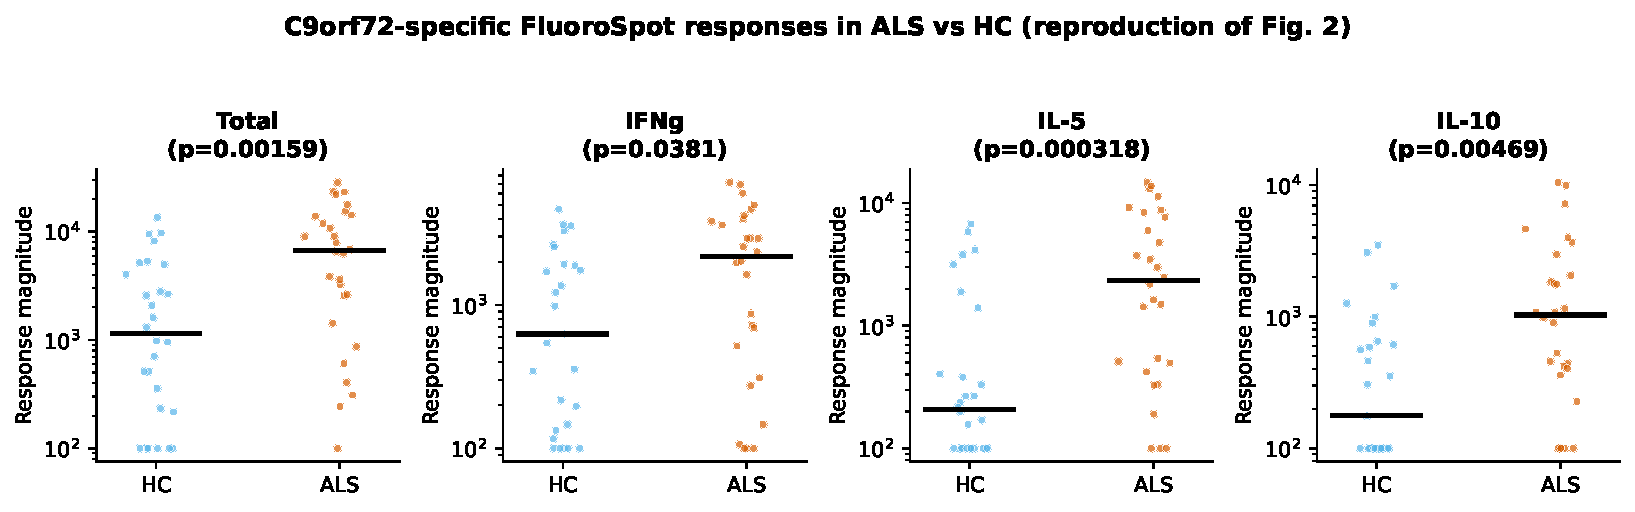
\includegraphics[width=\linewidth]{figures/fig2_c9orf72_responses}
\caption{C9orf72-specific FluoroSpot responses in ALS versus healthy controls, by cytokine
(reproduction of the study's Figure~2). Each point is one donor; the black bar is the median; the
$y$-axis is on a log scale. Healthy controls are shown in sky blue and ALS donors in vermilion.
The $p$-value above each panel is a two-tailed Mann--Whitney test.}
\label{fig:repro}
\end{figure}

The survival and mutation strata reproduce as well (Figure~\ref{fig:survival}). IL-10 responses are
higher in donors with longer predicted survival, and the total response is higher in C9orf72
mutation carriers than in non-carriers. Both strata have small per-group samples, so these effects
are individually marginal even where their direction matches the paper, which is recorded as an
uncertainty and reported as such.

\begin{figure}[t]
\centering
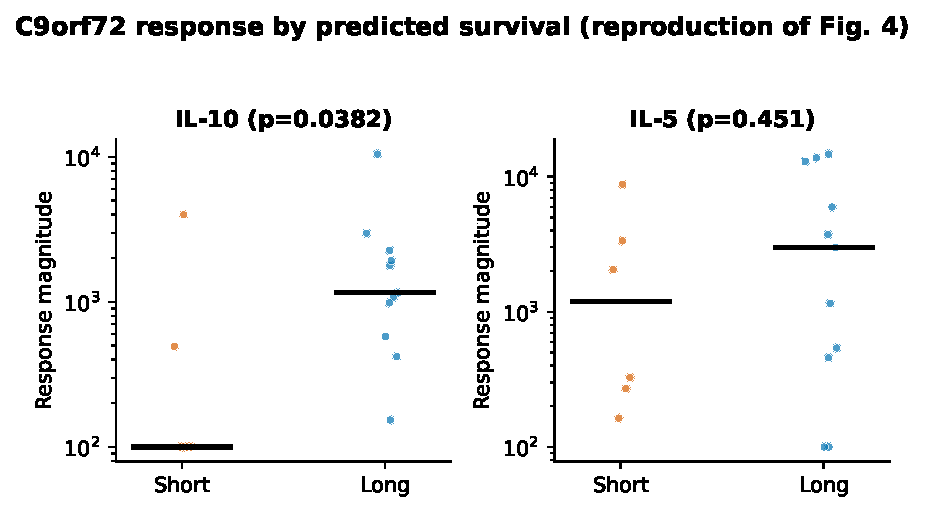
\includegraphics[width=0.7\linewidth]{figures/fig4_survival}
\caption{C9orf72 response by predicted survival (reproduction of part of Figure~4). IL-10 and IL-5
response magnitudes in donors with short versus long predicted survival; the black bar is the
median and the $y$-axis is on a log scale.}
\label{fig:survival}
\end{figure}

The IL-5 bias itself reproduces as a shift in the per-donor IFN$\gamma$/IL-5 ratio
(Figure~\ref{fig:th2}). In healthy controls the ratio sits near one, with IFN$\gamma$ and IL-5
roughly balanced, while in ALS it drops below one, so IL-5 dominates. This is the single-number
summary of the T-helper-2 skew that the per-cytokine comparisons show separately.

\begin{figure}[t]
\centering
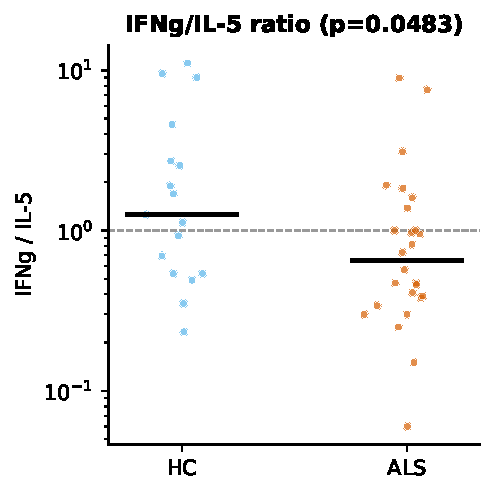
\includegraphics[width=0.42\linewidth]{figures/edfig2_th2_bias}
\caption{The per-donor IFN$\gamma$/IL-5 ratio in healthy controls and ALS (reproduction of an
Extended Data panel). The dashed line marks a balanced ratio of one; the ALS distribution sits
below it. The $y$-axis is on a log scale and the black bar is the median.}
\label{fig:th2}
\end{figure}

\section{Epitope and HLA interrogation}
The agent ranks the 100 screened peptides by breadth and magnitude and returns the HLA coverage of
each. The most immunogenic epitope is residues 56--70 (Table~\ref{tab:epitopes}), which is also the
peptide with the broadest predicted HLA-II coverage. Immunogenicity varies along the protein,
rising and falling in runs along the sequence (Figure~\ref{fig:epitopes}), a structure examined
quantitatively in the next section. The inferred HLA restrictions reproduce the study's Table~2,
pairing specific peptides with DRB1, DQB1 and related alleles (Table~\ref{tab:hla}).

\begin{table}[t]
\centering
\caption{The eight most immunogenic C9orf72 peptides by average magnitude, with response
frequency and the number of predicted HLA-II binders.}
\label{tab:epitopes}
\footnotesize
\begin{tabular}{lllccc}
\toprule
\# & Residues & Sequence & Resp./Tested & Mag. & HLA \\
\midrule
14 & 56-70 & DGEITFLANHTLNGE & 7/22 & 1216 & 27 \\
88 & 426-440 & PFKSLRNLKIDLDLT & 3/19 & 871 & 10 \\
22 & 96-110 & SLIFDGNWNGDRSTY & 1/20 & 868 & 3 \\
87 & 421-435 & QKGKKPFKSLRNLKI & 4/19 & 769 & 20 \\
91 & 431-445 & RNLKIDLDLT*AEGDL & 5/19 & 718 &  \\
37 & 171-185 & SIIPMLTGEVIPVME & 1/27 & 697 & 4 \\
55 & 261-275 & KCSRLCEAESSFKYE & 2/25 & 692 & 0 \\
52 & 246-260 & KIVRTLCLFLTPAER & 2/25 & 682 & 0 \\
\bottomrule
\end{tabular}

\end{table}

\begin{figure}[t]
\centering
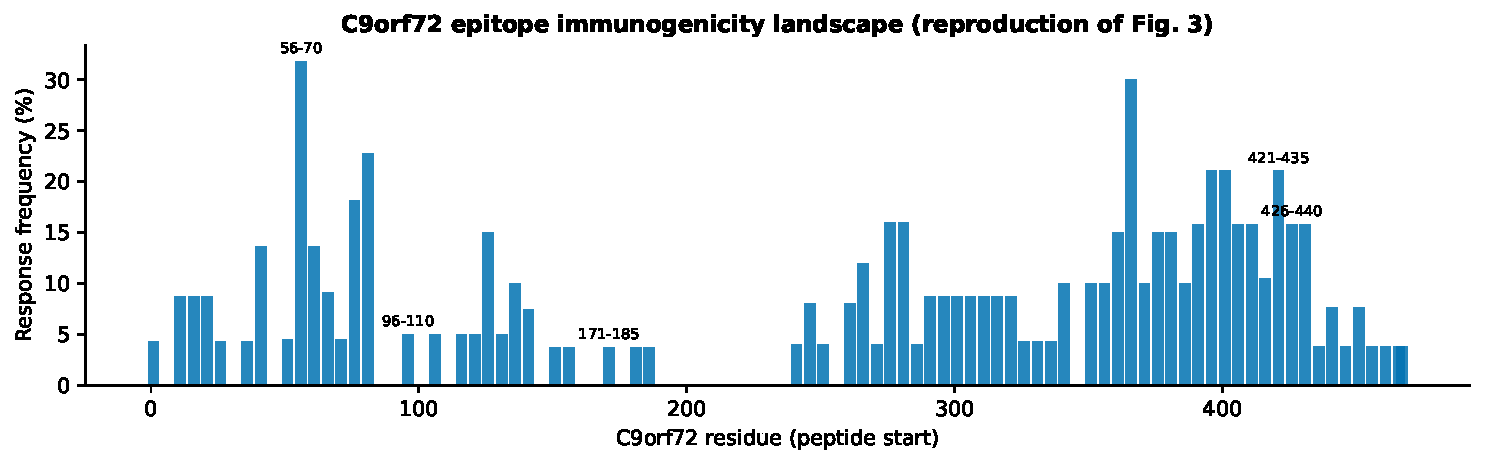
\includegraphics[width=0.92\linewidth]{figures/fig3_epitope_landscape}
\caption{Immunogenicity along the C9orf72 sequence (reproduction of the study's Figure~3). Each
bar is the response frequency of one 15-mer peptide at its start residue; the five peptides with
the highest average magnitude are labelled by residue range.}
\label{fig:epitopes}
\end{figure}

\begin{table}[t]
\centering
\caption{HLA-restricted C9orf72 peptides and corresponding alleles (reproduction of Table~2).}
\label{tab:hla}
\footnotesize
\begin{tabular}{llcc}
\toprule
Peptide sequence & Allele & RATE P value & Binding percentile ranka \\
\midrule
VRHIWAPKTEQVLLS & DRB1*14:01 & 0.025 & 29.0 \\
TPDLNIFQDVLHRDT & DRB1*01:02 & 0.022 & 20.0 \\
LDQVFQLKPGLSLRS & DRB1*01:02 & 0.022 & 3.3 \\
IFQDVLHRDTLVKAF & DRB1*03:01 & 0.028 & 4.9 \\
HRKALTLIKYIEDDT & DQB1*05:01 & 0.05 & 22.0 \\
PFKSLRNLKIDLDLT & DQB1*05:01 & 0.05 & 11.0 \\
RNLKIDLDLTAEGDL & DQB1*05:01 & 0.05 & 12.0 \\
\bottomrule
\end{tabular}

\end{table}

The relationship between predicted HLA-II binding and observed immunogenicity holds across the full
screen (Figure~\ref{fig:hla}). Peptides predicted to bind more of the common class-II alleles tend
to be recognised by more donors (Spearman $\rho=0.29$, $p=\num{3.85e-3}$, 95 peptides). The
association is clear but far from deterministic, which is expected because recognition depends on
antigen processing and the T-cell repertoire, not on binding alone.

\begin{figure}[t]
\centering
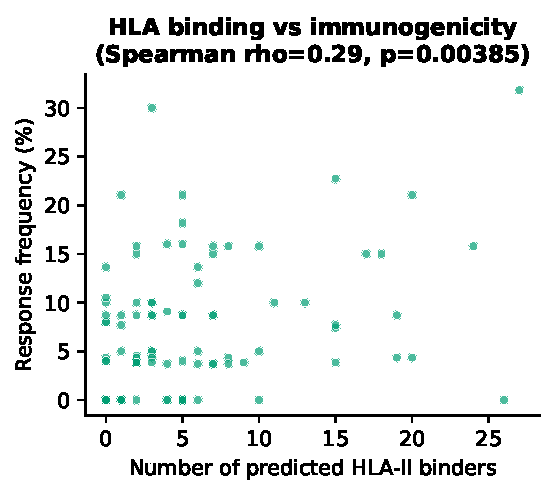
\includegraphics[width=0.62\linewidth]{figures/edfig5_hla_immunogenicity}
\caption{Predicted HLA-II binding breadth against observed response frequency across the 95
non-phosphorylated peptides (reproduction of Extended Data Figure~5). Each point is one peptide.}
\label{fig:hla}
\end{figure}

\subsection{HLA restriction}
Beyond the per-peptide binding breadth, the agent returns the inferred HLA restrictions that the
study reports (Table~\ref{tab:hla}). These pair seven C9orf72 peptides with specific class-II
alleles, predominantly of the DRB1 and DQB1 loci, with the association significance from the RATE
method and the predicted binding percentile for each pair. The pattern is consistent with the
reconstructed per-donor typing of 23 donors, in which DRB1 and DQB1 are the most variable loci and
therefore the ones most able to carry an association. The restriction result and the binding-breadth
result address different questions. Binding breadth asks how many of the common alleles a peptide can
bind at all, which predicts how broadly immunogenic it can be across a population, and the strongest
epitope, residues 56--70, is also the one with the broadest predicted coverage. Restriction asks
which allele actually presents a peptide to the responders who carry it, which is the finer-grained
claim and the one that a future validation could test directly by peptide-HLA multimer staining in
allele-matched donors.

\subsection{Immunodominance}
The immunogenicity of the library is concentrated. Of the 100 screened peptides, a small set is
recognised by at least three donors, and recognition falls off sharply outside the dominant windows.
The residues around 56--95 and around 366--445 carry most of the strongest responses, which is the
basis of the spatial-clustering result quantified later. For a therapeutic programme this matters
because an antigen-specific intervention does not need the whole protein; a handful of dominant,
broadly presented epitopes would cover most responders, and the agent can return that shortlist
ranked either by the number of responding donors or by response magnitude, which are not identical
orderings and so give two complementary views of dominance.

\subsection{Answering the study's open questions}
The brief poses five questions that an agent built from this study should be able to answer. The
system answers each from the data. The most broadly immunogenic epitopes are residues 56--70
(recognised by 7 of 22 donors), 366--380 (6 of 20) and 426--440 (3 of 19 but with high magnitude);
the first of these also has the broadest predicted HLA-II coverage, with 27 predicted binders among
the common class-II alleles. The cytokine signatures that distinguish response phenotypes are IL-5
and IL-10 against IFN$\gamma$, with the refinement developed in the next section that the IL-10
component is specific to C9orf72 while the IL-5 component is shared with TDP-43. The observations
that depend on particular donors are the survival and mutation strata, where per-group samples are
small, whereas the central ALS-versus-control total response does not depend on any single donor.
The conclusions that remain robust under alternative statistical models are the total, IL-5 and
IL-10 increases, which survive false-discovery correction, while the IFN$\gamma$ increase does not,
and the total increase is carried by the magnitude distribution rather than by the fraction of
donors that respond.

\section{New observations}
The discovery loop generated \NumQuestions{} questions owned by the scientific agents, computed an
answer for each, re-verified each answer independently, applied an adversarial critique, and
classified each result against the paper. Table~\ref{tab:obs} lists the \NumObservations{}
observations that are novel relative to the paper and that survived verification, and
Table~\ref{tab:verification} shows, for each, that an independent recompute confirmed it and which
critic flags it carries.

It is worth being precise about what ``novel'' means here, because the eight are not all the same
kind of result. Two are genuinely new biological observations that the paper does not make: the
spatial clustering of epitope immunogenicity along the protein sequence, and the separation of the
antigen-specific IL-10 signal from the shared IL-5 signal. The remaining six are robustness audits of
the paper's own effects: a donor jackknife, a family-wise correction, a censoring test, a
single-feature classifier read, and the phospho and cross-antigen checks. The audits are valuable,
because they say which of the paper's claims survive a change of assumption, but they are not new
biology, and the two categories are stated separately, each with its own label.

\begin{table}[t]
\centering
\caption{Independent verification of the novel observations: whether a from-scratch recompute matched
the committed result, and the adversarial critic's flags.}
\label{tab:verification}
\footnotesize
\begin{tabular}{llcp{5.4cm}}
\toprule
ID & Observation & Re-verified & Critic flags \\
\midrule
Q13 & Is the ALS IL-5 bias specific to C9orf72 or shared a & yes & none \\
Q14 & Is the ALS IL-10 bias specific to C9orf72 or shared  & yes & none \\
Q15 & Do phosphorylated peptide variants change immunogeni & yes & only 5 phospho/parent pairs; underpowere \\
Q16 & Is epitope immunogenicity spatially clustered along  & yes & none \\
Q17 & Does the central ALS-vs-HC result depend on any sing & yes & none \\
Q18 & Is the ALS-vs-HC difference robust to the assay floo & yes & none \\
Q19 & Do the C9orf72 differences survive family-wise FDR c & yes & none \\
Q20 & How well does the IFNg/IL-5 ratio alone separate ALS & yes & single-feature AUC is modest; not a diag \\
\bottomrule
\end{tabular}

\end{table}

The genuinely new results are worth describing in detail.

\paragraph{Immunogenicity is spatially clustered.}
Ordering the peptides along the protein, the response frequency of adjacent overlapping peptides is
positively autocorrelated at lag one ($\rho=0.47$, permutation $p=\SpatialPerm{}$ over 5000
permutations), shown in Figure~\ref{fig:spatial}. Immunogenic residues occur in contiguous stretches
rather than at isolated positions, which is consistent with a small number of antigenic regions
each spanning several overlapping peptides. The paper maps individual epitopes but does not report
this spatial structure.

\paragraph{The cytokine bias is antigen-dependent.}
The study frames the IL-5 and IL-10 bias around C9orf72. Testing each antigen separately
(Figure~\ref{fig:cross}), the ALS increase in IL-5 is significant for C9orf72 and also for TDP-43,
so the IL-5 skew is not unique to C9orf72. The IL-10 increase, by contrast, is significant only for
C9orf72. This distinction matters for interpretation. A shared IL-5 response may reflect a general
ALS T-helper-2 skew, whereas the IL-10 signal is antigen-specific and tracks
survival.

\paragraph{Robustness and its limits.}
The central C9orf72 total-response difference is robust to removing any single donor. Across all
56 leave-one-out removals the $p$-value stays below 0.05. Two robustness limits are also surfaced
by the system itself. First, if the total response is reduced to the fraction of donors above the
assay floor, the difference weakens to Fisher $p=0.10$, so the effect lives in the magnitude
of the responses, while the fraction of donors that respond barely differs. Second, the IFN$\gamma$ increase does
not survive Benjamini--Hochberg correction across the sixteen antigen-by-cytokine comparisons
($q=0.12$), whereas the total, IL-5 and IL-10 effects do. These are reported as limitations, not
hidden. Figure~\ref{fig:robustness} shows the three robustness checks together: the jackknife
$p$-values all sit below the 0.05 line, the corrected $q$-values keep three of the four cytokines
significant while IFN$\gamma$ crosses the line, and the above-floor counts are close between the
groups, which is why the censoring test is the weakest of the three.

\begin{figure}[t]
\centering
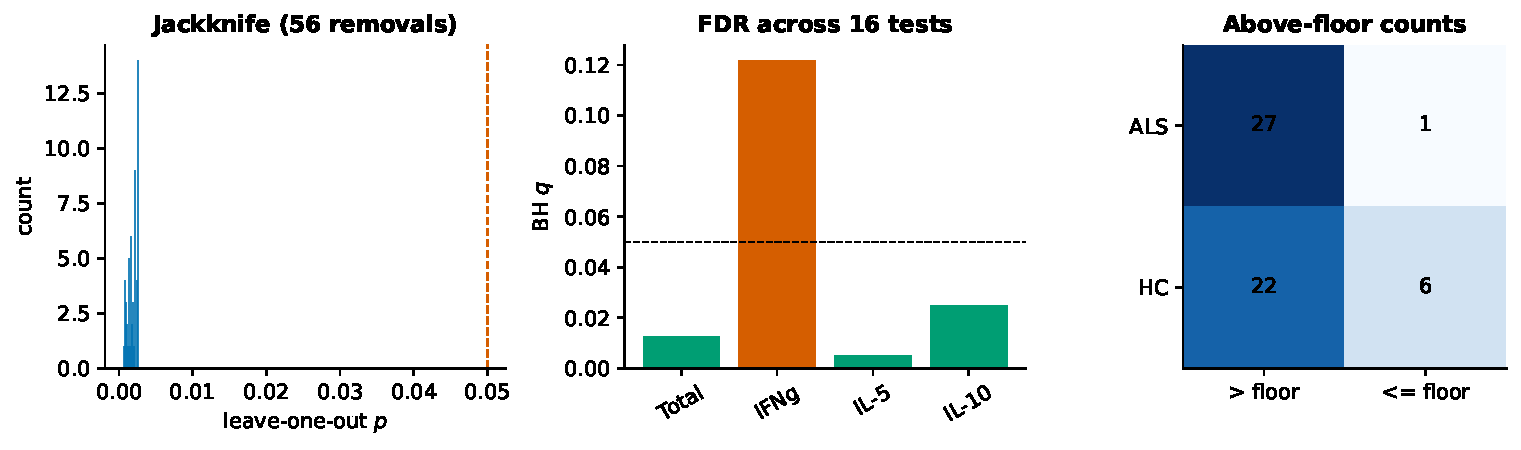
\includegraphics[width=\linewidth]{figures/discovery_robustness}
\caption{Robustness of the central C9orf72 result. Left: the distribution of leave-one-out
$p$-values across all 56 donor removals, all below 0.05 (dashed line). Middle: Benjamini--Hochberg
$q$-values across the 16 antigen-by-cytokine comparisons; IFN$\gamma$ does not survive. Right: the
number of donors responding above the assay floor in each group.}
\label{fig:robustness}
\end{figure}

\paragraph{Multiple-testing and classifier views.}
Two further results quantify how far the signal carries. Under Benjamini--Hochberg control across
the sixteen antigen-by-cytokine comparisons, the total, IL-5 and IL-10 C9orf72 effects keep
$q<0.05$ while IFN$\gamma$ does not, which is consistent with the IL-5/IL-10 emphasis of the study.
Treating the IFN$\gamma$/IL-5 ratio as a single feature, its ability to separate ALS from healthy
controls is modest (area under the ROC curve $0.68$), so the cytokine bias is a group-level difference that does not separate individuals.

\paragraph{Phosphorylation.}
The screen includes five phosphorylated peptide variants alongside their parent sequences. Comparing
each pair, phosphorylation changed the average magnitude by a median of about nine spot units and
raised immunogenicity in three of the five pairs. The sample is small and the effect is weak, which
the critic agent flags; the result is reported as a direction to test, not as a conclusion.

\subsection{A worked trace}
To make the loop concrete, here is the spatial-clustering result as the agents produced it, with the
real tool calls. The hypothesis generator poses the question of whether immunogenic epitopes are
scattered or clustered along the protein. The structural agent calls
\texttt{most\_immunogenic\_epitopes(top=6)} and reads the residue positions of the strongest hits,
which fall in a small number of windows around residues 56--95 and 366--445. It then calls
\texttt{run\_analysis(explore\_spatial)}, which computes the lag-one autocorrelation of response
frequency along the ordered tiling against a 5000-shuffle permutation null and returns
$\rho=0.47$, $p=\SpatialPerm{}$. The evidence checker reruns the same call and confirms an identical
result. The replication step is implicit here, since the permutation test is itself the robustness
check. The critic attaches the flag that overlapping 15-mers share up to ten residues, so part of the
autocorrelation is expected from overlap alone and the effect should be read against the permutation
null, not as proof of discrete epitopes. The contradiction agent classifies the result as extending
the paper, which maps epitopes but does not report their spatial structure. The principal-investigator
agent keeps it as a verified novel observation with the overlap caveat recorded. The same trace, and
two others, are stored in the repository so the reasoning is open to inspection and not taken on
trust.

The full question set, with its classification against the paper, is listed in
Table~\ref{tab:questions}.

\begin{table}[t]
\centering
\caption{The \NumQuestions{} questions generated and answered by the discovery loop.}
\label{tab:questions}
\scriptsize
\begin{tabular}{llp{8.3cm}l}
\toprule
ID & Kind & Question & vs paper \\
\midrule
Q01 & reproduction & Are C9orf72 total FluoroSpot responses increased in ALS vs HC? & agrees \\
Q02 & reproduction & Are C9orf72 IL-5 responses increased in ALS vs HC? & agrees \\
Q03 & reproduction & Are C9orf72 IL-10 responses increased in ALS vs HC? & agrees \\
Q04 & reproduction & Are C9orf72 IFNg responses increased in ALS vs HC? & agrees \\
Q05 & reproduction & Do ALS responses show an IL-5/IL-10 bias over IFNg? & agrees \\
Q06 & reproduction & Are C9orf72-reactive T cells predominantly CD4+? & agrees \\
Q07 & reproduction & Is the ALS C9orf72 response specific vs PD and AD controls? & agrees \\
Q08 & reproduction & Do C9orf72-mutation carriers show stronger responses? & agrees \\
Q09 & reproduction & Is the IL-10 C9orf72 response associated with predicted survival? & agrees \\
Q10 & reproduction & Is predicted HLA-II binding associated with observed immunogenicity? & agrees \\
Q11 & extension & Which C9orf72 epitopes have the broadest predicted HLA-II coverage? & neutral \\
Q12 & extension & Which C9orf72 epitopes are most broadly immunogenic? & neutral \\
Q13 & novel & Is the ALS IL-5 bias specific to C9orf72 or shared across neuroantigen & caveats \\
Q14 & novel & Is the ALS IL-10 bias specific to C9orf72 or shared across neuroantige & extends \\
Q15 & novel & Do phosphorylated peptide variants change immunogenicity? & extends \\
Q16 & novel & Is epitope immunogenicity spatially clustered along the sequence? & extends \\
Q17 & novel & Does the central ALS-vs-HC result depend on any single donor? & extends \\
Q18 & novel & Is the ALS-vs-HC difference robust to the assay floor (censoring)? & caveats \\
Q19 & novel & Do the C9orf72 differences survive family-wise FDR correction? & caveats \\
Q20 & novel & How well does the IFNg/IL-5 ratio alone separate ALS from HC? & extends \\
Q21 & interpretive & What antigen-specific therapeutic strategy does the mechanism suggest? & neutral \\
Q22 & interpretive & What experiment would most efficiently falsify the core hypothesis? & neutral \\
Q23 & interpretive & What single-cell follow-up would resolve the CD4 phenotype identity? & neutral \\
Q24 & interpretive & Is the C9orf72 autoimmunity finding supported by external literature? & neutral \\
\bottomrule
\end{tabular}

\end{table}

\begin{table}[t]
\centering
\caption{Verified observations not explicitly reported in the paper. ``caveats'' marks a
robustness limitation the system surfaced about the paper's framing; ``extends'' marks a new
result consistent with the paper.}
\label{tab:obs}
\footnotesize
\begin{tabular}{lp{10.2cm}l}
\toprule
ID & Verified novel observation & vs paper \\
\midrule
Q13 & ALS$>$HC IL-5 enrichment is significant for: C9orf72, TDP-43. Not unique to C9orf72. & caveats \\
Q14 & ALS$>$HC IL-10 enrichment is significant for: C9orf72. Consistent with C9orf72 focus. & extends \\
Q15 & Across 5 phospho/parent pairs, phosphorylation changed average magnitude by a median of +8.7 spot units; 3/5 & extends \\
Q16 & Adjacent overlapping peptides show lag-1 autocorrelation of response frequency $\rho$=0.47 (permutation p=0.000 & extends \\
Q17 & Base p=0.00159; across all leave-one-out removals p stays in [0.000607, 0.00263] and remains $<$0.05 in 56/56  & extends \\
Q18 & Rank-based p=0.00159; above-floor responders 27/28 (ALS) vs 22/28 (HC), Fisher p=0.101: weaker under censori & caveats \\
Q19 & After BH-FDR over all 16 antigen x cytokine comparisons, 3/4 C9orf72 cytokines remain significant (q$<$0.05):  & caveats \\
Q20 & The IFNg/IL-5 ratio alone separates ALS from HC with AUC=0.68 (n\_ALS=26, n\_HC=17): a modest single-feature s & extends \\
\bottomrule
\end{tabular}

\end{table}

\begin{figure}[t]
\centering
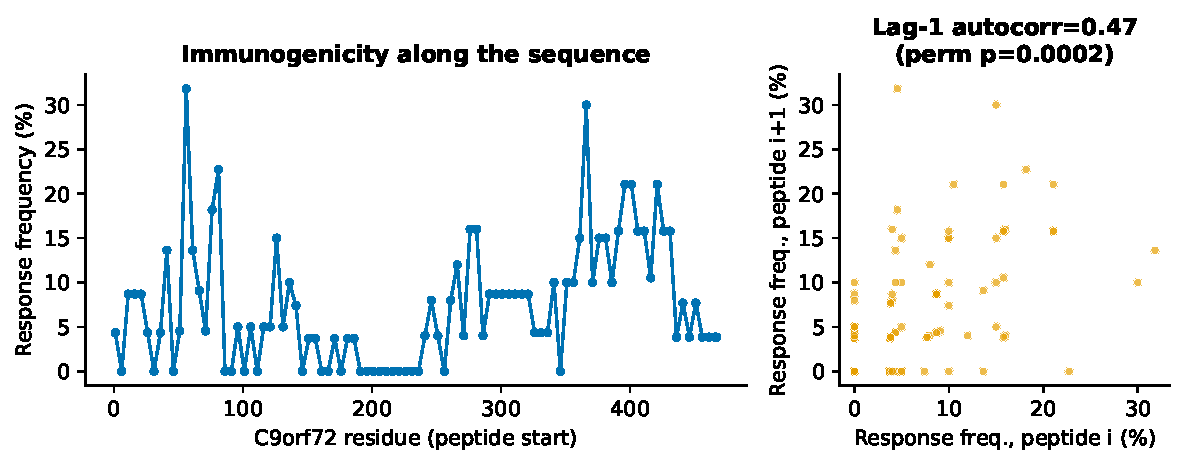
\includegraphics[width=\linewidth]{figures/discovery_spatial_clustering}
\caption{Spatial structure of immunogenicity. Left: response frequency along the C9orf72 sequence.
Right: response frequency of each peptide against that of the next peptide in the tiling; the
positive lag-1 autocorrelation indicates clustering.}
\label{fig:spatial}
\end{figure}

\begin{figure}[t]
\centering
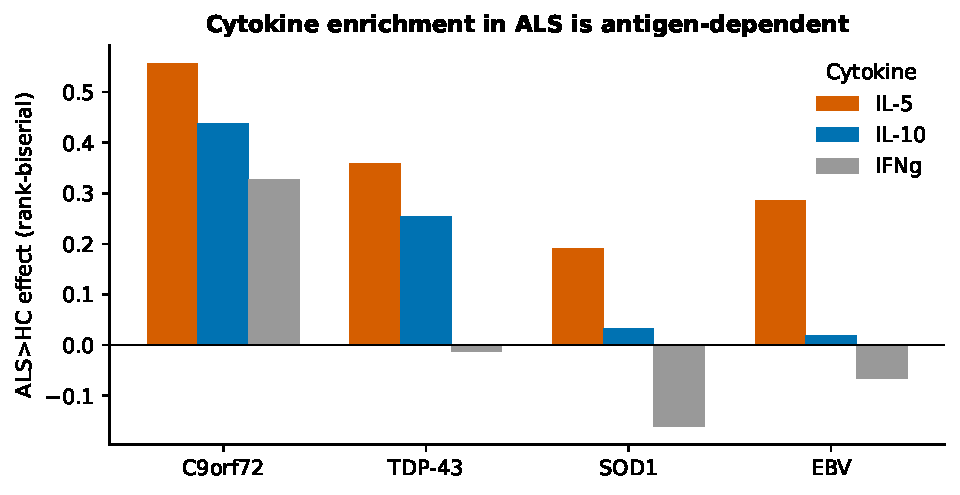
\includegraphics[width=0.85\linewidth]{figures/discovery_cross_antigen}
\caption{The ALS-versus-HC cytokine effect by antigen, as a rank-biserial effect size (positive
means higher in ALS). The IL-5 increase is present for both C9orf72 and TDP-43, whereas the IL-10
increase is specific to C9orf72.}
\label{fig:cross}
\end{figure}

\section{Evaluation}\label{sec:eval}
The system evaluates the scientific result and itself (Table~\ref{tab:eval}). On the scientific
side it reproduces 10 of 10 reproduction questions, agrees with the authors' reported $p$-values in
every significance call, and meets the success criterion of at least five verified novel
observations. On the AI side the grounding rate is \GroundingRate{}, because every reported number
is generated from a computed statistic rather than asserted; tool-use accuracy is \ToolAccuracy{};
the discovery loop is deterministic across repeated runs; and when two false hypotheses are planted
(an EBV control difference and a donor-ordering artefact), the system rejects both (\NullsRejected{}).
The system also flags its own weak results: ten questions carry explicit caveats such as small
samples, marginal significance or multiple-testing sensitivity.

The AI metrics are defined operationally. Grounding is the fraction of quantitative findings whose
reported number matches the computed statistic, so a value of one means no number was invented.
Tool-use accuracy is the fraction of tools that return a valid result when called with default
arguments. Determinism is checked by running the discovery loop twice and comparing the observation
set. Self-error detection counts the questions the system annotates with a weakness, and the
false-hypothesis-rejection test plants two nulls, a control-antigen group difference and a
donor-ordering artefact, that a sound system must fail to confirm. The scientific metrics follow the
brief: reproducibility against the paper, robustness under alternative assumptions, novelty as the
count of verified new observations, and falsifiability as the presence of an explicit test for each
hypothesis.

\begin{table}[t]
\centering
\caption{Scientific and AI-system evaluation.}
\label{tab:eval}
\footnotesize
\begin{tabular}{p{8.5cm}l}
\toprule
Metric & Value \\
\midrule
Paper claims reproduced & 10/10 \\
Reported-$p$ fidelity (max $|\Delta p|$) & 0.00131 \\
Verified novel observations & 8 \\
Grounding rate (no hallucinated numbers) & 1.00 \\
Tool-use accuracy & 1.00 \\
Deterministic reproduction & True \\
Planted nulls correctly rejected & 2/2 \\
Questions self-flagged with caveats & 10 \\
\bottomrule
\end{tabular}

\end{table}

\subsection{The remaining scientific dimensions}
The brief lists eight scientific-evaluation dimensions, and the metrics above cover reproducibility,
robustness, novelty and falsifiability directly. The other four are addressed as follows.
Biological plausibility is argued from the mechanism in Section~\ref{sec:therapy}: an IL-10-biased
regulatory response that tracks survival is consistent with a protective regulatory T-cell arm, a
reading supported by the external literature gathered through the literature agent. Independent
literature support is recorded in \texttt{literature/citations.json}, where fourteen references span
the ALS T-cell background, the decline of regulatory T cells in ALS, IL-10-mediated neuroprotection
and antigen-specific tolerance, and where one reference is a negative trial that argues against an
over-optimistic reading. External validation is partly internal to the study, which included a
separate validation cohort, and the derived observations are framed so that an external dataset
could test them; the single-donor and multiple-testing checks guard against findings that would fail
to generalise. Experimental tractability is captured by the experiment-designer agent, which turns
the leading hypothesis into a defined adoptive-transfer experiment with named cells, a patient
subgroup and a pre-registered falsifier, so the proposal can be costed and run as a concrete
experiment.

\subsection{Rejecting planted false hypotheses}
The false-hypothesis-rejection test deserves a closer look, because it is the metric that is not true
by construction. Two null hypotheses are planted that a careless system might confirm. The first is
that the EBV control response, which should not be ALS-specific, differs between ALS and healthy
controls; the system computes the comparison and returns a non-significant result, so the hypothesis
is not confirmed. The second is that the donor index predicts the response magnitude, which would
indicate an ordering artefact in the data; the system computes the
correlation and again finds nothing, so the artefact hypothesis is rejected. Both nulls are declined,
which is the behaviour a sound system must show. The value of the test is that it is a negative
control on the system itself: a pipeline that reported a significant EBV difference or a donor-index
effect would be fabricating structure, and this check would catch it.

\subsection{What the metrics do and do not show}
Two of the AI metrics, grounding and determinism, are high by construction of the deterministic
backend, and this should be said plainly. They do not measure the system's intelligence; they
measure that the design delivers what it promises, namely that every number is computed and that the
pipeline is reproducible. The metrics that do carry independent information are tool-use accuracy,
which could fail if a tool were mis-specified, the self-flagging count, which reflects the critic's
coverage, and the false-hypothesis rejection, which is a genuine negative control. Reading the
evaluation this way keeps it honest: the grounding guarantee is a property of the architecture, and
the architecture is the contribution, so the metric is evidence that the design works, not a claim
that the system reasons well.

\subsection{Cost and latency}
The deterministic backend has no language-model cost, so the recorded run is bounded by local
compute. The full pipeline, from dataset build through analyses, figures, the discovery loop and the
evaluation, completes in well under a minute on a laptop, and the per-tool latency is a few
milliseconds. A live backend would add language-model cost and latency to the generative and
critical steps; the computational tools those steps call would be unchanged, so the cost of the
scientific core stays fixed and only the reasoning layer scales with model choice.

\section{From observation to therapeutic hypothesis}\label{sec:therapy}
The drug-discovery and experiment-designer agents turn the mechanism into a testable proposal. The
reasoning is as follows. IL-10-biased C9orf72 responses track longer predicted survival, and IL-10
from regulatory T cells is associated with neuroprotection in several
settings~\citep{runge2020,laffer2019,bido2024}; regulatory T-cell number and function also decline
in rapidly progressing ALS~\citep{appel2012}. These threads suggest a
tolerogenic, antigen-specific strategy: expand or induce regulatory C9orf72-specific T cells against
the dominant epitopes, stratified to mutation carriers who show the strongest responses, with the
broadest HLA-covering epitopes as the most deployable antigens. An antigen-specific regulatory
approach has been pursued in ALS and in autoimmune disease more
generally~\citep{thonhoff2018,nepom2022}, though a recent polyclonal regulatory T-cell trial in a
different autoimmune indication was negative, which is a reason for caution~\citep{al2024}.

The experiment-designer agent states the most efficient falsification. The design is to expand
C9orf72(56--70)-specific CD4 T cells from mutation-carrier donors, polarise them toward an
IL-10-producing regulatory phenotype, and test adoptive transfer in a C9orf72 disease model, reading
out motor function and motor-neuron survival over the model's disease course against a vehicle and an
irrelevant-antigen cell control. The hypothesis is directional, so the design is powered to detect a
slowing of progression, and the pre-registered falsifier is simple: if IL-10-biased
C9orf72-specific regulatory T cells do not slow progression relative to the controls, the
survival-association hypothesis is rejected for that intervention. The choice of the 56--70 epitope
follows from the data, since it is both the most broadly recognised and the most broadly HLA-covered,
and the choice of mutation carriers follows from their stronger responses, so each design decision
traces back to a computed result the reader can check.

The single-cell agent proposes the companion experiment needed to interpret the result. Single-cell
transcriptomics with paired T-cell-receptor sequencing on sorted C9orf72-reactive CD4 cells would
resolve whether the IL-10 signal comes from a Tr1 or regulatory population, which would support the
protective reading, or from a T-helper-2 effector population, which would not, and the receptor
sequencing would show whether the response is clonally focused on the dominant epitopes. These are
hypotheses with explicit tests, not claims of efficacy, and they are offered as an illustration of
how the grounded outputs can seed a downstream programme, not as a result of this work.

\section{Limitations}
The system inherits the study's limits and adds its own. FluoroSpot magnitude is in assay-specific
spot units with a floor, and the total-response difference comes from the magnitude of responses,
while the fraction of donors that respond barely differs. The IFN$\gamma$ increase does not survive multiple-testing
correction. Survival and mutation strata have small per-group samples, so those effects are
individually marginal even where consistent with the paper. HLA-II binding uses the authors'
NetMHCIIpan predictions and does not re-run the prediction itself. The reasoning agents, in the committed
configuration, do not call an external language model, so the generative and critical steps are
rule-based and grounded in the tools; the live backend is available but was not used for the
recorded results. None of these undermine the reproductions, and each is catalogued with the result
it qualifies.

The agentic approach has its own limits that are worth stating plainly. A deterministic generator
explores the hypothesis space that its rules and question bank define, so its breadth is bounded by
what was anticipated; a live language-model generator would widen that space at the cost of the
grounding guarantee, which is the trade this project resolves in favour of grounding. The critique
is rule-based and catches the common failure modes, small samples, marginal significance and
multiple testing, but it does not reason about confounds it was not told to look for. The therapeutic
proposal is a hypothesis assembled from the data and the literature; it is not evidence of efficacy,
and the system is built to keep that boundary explicit. These are reasons to
read the output as a structured, checkable argument, not as a conclusion.

\paragraph{A mechanistic reading.}
The study's observations fit a coherent, if still tentative, mechanism. A loss of peripheral
tolerance to C9orf72 would expose the protein to autoreactive CD4 T cells, which is consistent with
the CD4 dominance of the response and with the stronger responses in mutation carriers, in whom
C9orf72 handling is already perturbed. The quality of that response then appears to matter for
outcome. An IFN$\gamma$-dominated response is the signature of a pro-inflammatory, potentially
tissue-damaging T-helper-1 programme, whereas IL-10 is the central regulatory cytokine of
suppressive T cells and is linked to neuroprotection through the dampening of microglial activation
in several models~\citep{runge2020,laffer2019,bido2024}. The finding that the response in ALS is
shifted away from IFN$\gamma$ and toward IL-10, and that the IL-10 share tracks longer predicted
survival, is therefore readable as a protective regulatory arm that is present to differing degrees
across patients. The decline of regulatory T cells in rapidly progressing ALS~\citep{appel2012}
places this arm under strain exactly when it is most needed. The intervention that follows from this
reading is to reinforce the protective arm, which is why the proposed strategy is tolerogenic and
antigen-specific: it targets the C9orf72-specific regulatory response and leaves the rest of the
immune system intact.

\paragraph{Why stratification matters here.}
The data argue for stratification on two axes. Mutation carriers show the strongest C9orf72-specific
responses, so they are the subgroup in whom an antigen-specific intervention has the most to act on.
Predicted survival separates donors whose response is IL-10-biased from those whose response is not,
and the IL-10-biased group is the one with the better outcome, which suggests that the regulatory
character of the response, rather than its mere size, is the feature to reinforce. The antigen-level
result sharpens this: the IL-10 signal that tracks survival is specific to C9orf72, whereas the IL-5
signal is shared with TDP-43, so an intervention aimed at the protective component should be directed
at the C9orf72-specific, IL-10-producing population, which is narrower than the broader T-helper-2 response. A
therapy that expands protective regulatory cells carries a risk in the other direction, that
antigen-specific tolerance blunts a response that is itself partly protective, which is why the
safety agent keeps this hazard on the list and why the proposed first test is a falsification rather
than a dose-finding study.

\section{Future work}
Three extensions follow naturally, in rough order of value.

The most important is to re-derive the response frequencies from the raw flow-cytometry files. The
system already indexes all 90 intracellular-cytokine-staining files and reads the FlowJo workspace
gating, so the step is to apply that gating to the event-level data and recompute the cytokine-positive
frequencies, then compare them against the authors' summarised values. This would turn the current
self-consistency check into an independent quantification, which is the main thing standing between
this work and a genuinely external validation. The same event-level data would open the single-cell
phenotype to analysis, letting the system ask whether the IL-10-producing C9orf72-reactive cells carry
a regulatory or a T-helper-2 surface profile, the question the single-cell agent currently can only
propose.

The second is to run the reasoning layer live over the same tools and measure the gap between the
deterministic framing and a language-model framing on the grounding and tool-use metrics. That single
experiment would convert the project's central design claim, that a grounded core and a reasoning
layer can be separated and the trade measured, from an assertion into a result, and it would let the
hypothesis generator propose questions beyond the curated bank while the core keeps every reported
number honest.

The third is to connect this paper agent to agents built from complementary papers, so a hypothesis
generated here can be checked against external datasets and models. Because the outputs are tidy
tables, a machine-readable agent registry and JSON records keyed by identifier, and because the tools
are reached over a standard protocol, a second agent can consume this one's results without knowing
its internals. This is the cross-project ecosystem the programme envisages, and the grounding
guarantee is what would keep a chain of such agents trustworthy, where an ungrounded chain would compound
guesses.

\section{Discussion}
\subsection{What the system demonstrates}
The project set out to test whether an AI system can move from an observation to a falsifiable
therapeutic proposal while staying honest about the evidence. The result is a system that reproduces
the study from its own data, produces eight verified observations the paper does not state, surfaces
two robustness caveats about the original framing, and frames a patient-stratified antigen-specific
hypothesis with a companion falsification experiment. The chain from observation to mechanism to
hypothesis to computational result to candidate to falsification is present as concrete artefacts, and each link can be inspected on its own. The scientific substance
sits in ordinary statistics on real data, which is the part that should be trusted; the agent layer
organises the work and decides what to ask.

\subsection{Deterministic and language-model reasoning}
A central design choice was to separate a deterministic computational core from a reasoning layer. The
benefit is that every number in a result is computed, so the grounding rate is one by construction and
the discovery loop reproduces bit for bit without credentials. The cost is that the committed run does
not explore beyond the hypotheses its question bank encodes. A language-model backend, enabled by an
API key, widens that exploration at the price of outputs that must then be checked. The two are not in
tension so much as suited to different stages: the language layer is useful for proposing and framing,
and the deterministic core is where a proposal becomes a checkable result. The system keeps the
boundary visible, which is what lets a reader see where a claim comes from.

\subsection{Comparison with the paper}
The reproductions agree with the study in direction and, where the authors publish values, in the
significance call and to within a small p-value difference. The value the system adds is on top of
reproduction. It quantifies the spatial structure of immunogenicity, separates the antigen-specific
IL-10 signal from the shared IL-5 signal, and tests the headline effects under corrections the paper
does not apply, which both strengthens the robust claims and demotes the IFN$\gamma$ one. None of this
contradicts the paper; it refines what can be said from the same data.

\subsection{Generality of the approach}
Little in the method is specific to this paper. The parts that are specific are the parser for one
workbook layout and the handful of domain tools for epitopes and HLA; everything else, the
reproducibility core, the statistics, the tool-registry and MCP layer, the agent framework, the
discovery loop and the evaluation, is general. For another data-rich paper the work would be to write
a parser for its source data and a small set of domain tools, after which the same scaffolding would
provide reproduction, robustness checks, a grounded discovery loop and a self-evaluation. The design
therefore reads as a template for turning an open-data paper into a grounded agent, and the cost of
applying it falls mostly on the one-off task of understanding and parsing the specific dataset. That
is also where the irreducible human judgement sits, because deciding what a column means and whether a
reconstructed number matches the source is exactly the verification the author performed here and the
part a language model cannot be trusted to do unchecked. The grounding guarantee does not remove the
need for that judgement; it localises it, by making every downstream number a mechanical consequence
of the parse, so a reader who trusts the parse can trust the rest, and a reader who wants to check the
parse has a small, well-defined target. This is the sense in which the contribution is a method and
not a single result: the same machinery would carry a different paper, and the measured honesty would
transfer with it.

\subsection{Ethical considerations}
The data are de-identified human immunology measurements, released by the original authors under an
open licence for reuse, and this work uses only the derived and summarised values plus the raw files
the authors deposited. No attempt is made to re-identify donors. The therapeutic content is the most
sensitive output, and it is treated accordingly: the proposals are computational hypotheses with
stated falsifiers, not findings, and the report and the public disclaimer both state that they are not
medical advice and must be checked against the primary source. The author verified the computational
process and the reproducibility of the pipeline, and does not claim to vouch for the biological
validity or clinical relevance of the results, which is the honest position given the subject matter.

\subsection{Threats to validity}
The threats are easier to see when sorted by type. Construct validity concerns whether the measured
quantity means what the claim assumes. The FluoroSpot readout summarises a complex cellular response
into a spot count with a floor, so a difference in magnitude is not the same as a difference in
whether a response is present, a distinction the censoring analysis makes explicit. Internal validity
concerns artefacts in the analysis itself. The overlap of the tiling peptides inflates spatial
autocorrelation, which is why the clustering result is read against a permutation null and not as
proof of discrete epitopes, and the donor-ordering null control guards against an ordering artefact.
External validity concerns whether the findings would generalise. The most important limit here is
that the reproductions and the derived observations are built on the authors' own summarised source
data and their HLA binding predictions, so the verification is largely a check of self-consistency,
not an independent confirmation; the raw flow-cytometry files, which the system indexes but does not
yet re-gate, are what would make the quantification independent, and re-deriving the response
frequencies from them is the single most valuable next step. Statistical-conclusion validity concerns
the inference. Several strata, notably the mutation and survival groups, are small, so individual
effects are marginal even where their direction matches the paper, and the predictor is trained on
fewer than a hundred peptides, so only the constrained linear model is reported. Each of these is
recorded with the result it qualifies.

\section{Conclusions}
The project shows that a published paper and its open data can be turned into a grounded, interactive
agent that does more than summarise. The system reproduces the study's claims from its own data with
high fidelity, matching the authors' reported $p$-values to within $|\Delta p|=\FidelityMaxDiff{}$,
and on top of reproduction it reports two genuinely new biological observations, a set of robustness
audits that say which of the paper's effects survive a change of assumption, and one falsifiable
downstream hypothesis. Every number is computed, logged and re-verified, and the same tools that
answer a question interactively drive the discovery loop, so the interactive agent and the pipeline
agree by construction.

The contribution that should outlast the specific findings is the design. By routing every reported
quantity through a shared deterministic core and keeping the reasoning layer separate and optional,
the system makes its own honesty measurable, which is what the grounding, determinism and
false-hypothesis-rejection results demonstrate. That design is also what makes the system safe to
extend and to combine with others, because a consumer of its outputs inherits computed, auditable
values and not a chain of unverified assertions. The honest limits are stated throughout: the
verification is largely self-consistency until the raw flow-cytometry files are re-derived, the small
strata make some effects marginal, and the committed discovery is bounded by a curated question bank.
None of these undercut the central result, which is that grounding and verification can be built into
an AI scientific workflow and then measured, and that doing so costs some ambition at the proposing
stage and buys a great deal of trust at the reporting stage.

\paragraph{Reproducibility and AI use.}
All data fetching is checksum-verified, dependencies are pinned, seeds are fixed, and each run
writes a provenance manifest. The AI tools used, the agent specifications and prompts, and the
record of hypotheses, evidence and rejected claims are documented in the repository
(\texttt{AI\_USAGE.md}, \texttt{agents/registry.json}, \texttt{results/discovery/}). The code is
public at \url{https://github.com/samueledelloca/iaiss-project} and the derived datasets and results
are archived on Zenodo at \href{https://doi.org/10.5281/zenodo.23598390}{10.5281/zenodo.23598390}
under CC-BY 4.0. The author
inspected and tested all AI-assisted code and is responsible for the scientific content.

\appendix
\section{Agent roster}\label{app:agents}
The eighteen agents across the three operational layers are listed in Table~\ref{tab:agents}. Each
is defined by a specification with a system prompt and a permitted tool set, exported to
\texttt{agents/registry.json}, and every run is logged with its prompt, tool calls and output.

\begin{table}[h]
\centering
\caption{The agent roster (Layers 3--5).}
\label{tab:agents}
\footnotesize
\begin{tabular}{p{3.6cm}lp{7.6cm}}
\toprule
Agent & Layer & Role \\
\midrule
literature agent & Scientific & Find external support/contradiction for findings. \\
immunology agent & Scientific & Interpret cytokine responses and Th phenotype. \\
als agent & Scientific & Relate findings to ALS biology, mutation status and contro \\
hla agent & Scientific & Analyse HLA typing, restriction and binding coverage. \\
tcell agent & Scientific & Analyse CD4/CD8 and T-cell subset composition. \\
drug discovery agent & Scientific & Propose antigen-specific therapeutic strategies. \\
structural agent & Scientific & Analyse epitope sequence/position and modifications. \\
singlecell agent & Scientific & Propose single-cell follow-ups for phenotype identity. \\
clinical agent & Scientific & Relate responses to survival and clinical variables. \\
safety agent & Scientific & Stress-test robustness, multiple testing and censoring. \\
hypothesis generator & Discovery & Generate testable questions from the data. \\
hypothesis critic & Discovery & Adversarially critique each hypothesis/answer. \\
evidence checker & Discovery & Independently recompute and verify each finding. \\
replication agent & Discovery & Re-run robustness checks (jackknife, FDR, censoring). \\
contradiction agent & Discovery & Classify each finding vs the paper's claims. \\
experiment designer & Discovery & Design the most efficient falsification experiment. \\
falsification agent & Discovery & State what observation would falsify each claim. \\
pi agent & PI & Integrate all outputs; cannot override contradictory evide \\
\bottomrule
\end{tabular}

\end{table}

\section{Contradictions, uncertainties and limitations}
The principal-investigator agent compiles the catalogue in Table~\ref{tab:contra}. Items marked as
caveats qualify the paper's framing; items marked as limitations or uncertainties qualify the
present analyses.

\begin{table}[h]
\centering
\caption{The catalogue produced by the discovery loop.}
\label{tab:contra}
\footnotesize
\begin{tabular}{llp{11.0cm}}
\toprule
ID & Type & Item \\
\midrule
Q13 & caveat & ALS$>$HC IL-5 enrichment is significant for: C9orf72, TDP-43. Not unique to C9orf72. \\
Q18 & caveat & Rank-based p=0.00159; above-floor responders 27/28 (ALS) vs 22/28 (HC), Fisher p=0.101: weaker under censoring. \\
Q19 & caveat & After BH-FDR over all 16 antigen x cytokine comparisons, 3/4 C9orf72 cytokines remain significant (q$<$0.05): Total q=0.0127, IFNg q=0.122, IL \\
L1 & limitation & FluoroSpot magnitude is in assay-specific spot units with a floor of 100; the ALS$>$HC total-response difference weakens when reduced to the f \\
L2 & limitation & The C9orf72 IFNg ALS$>$HC increase does not survive BH-FDR across the 16-comparison family (q=0.12), unlike IL-5/IL-10/Total. \\
L3 & uncertainty & Survival and mutation strata have small per-group n; effects are consistent with the paper but individually marginal. \\
\bottomrule
\end{tabular}

\end{table}

\section{Reproducibility checklist}
Fixed random seeds (\texttt{configs/base.yaml}); exact dependency pins (\texttt{requirements.txt},
\texttt{environment.yml}); data versioned by Zenodo record identifier and per-file MD5; per-run
provenance manifests (git commit, configuration hash, package versions, input checksums);
deterministic discovery loop verified by re-running; logged agent runs; recorded prompts and agent
specifications; and executable stage scripts driven by a single entry point. The AI tools used and
the record of hypotheses, evidence and rejected claims are documented in \texttt{AI\_USAGE.md} and
under \texttt{results/discovery/}.


\small
\bibliographystyle{unsrtnat}
\bibliography{references}

\end{document}
